\documentclass[tc,oneside]{iiufrgs}

\usepackage[T1]{fontenc}        % pacote para conj. de caracteres correto
\usepackage[utf8]{inputenc}   % pacote para acentua\c c\~ ao
\usepackage{graphicx}           % pacote para importar figuras
\usepackage{times}              % pacote para usar fonte Adobe Times
\usepackage{multirow}
\usepackage{subfigure}
\usepackage{listings}
\usepackage{scalefnt}
\usepackage[brazilian]{babel}
\usepackage{tabularx}
%\usepackage{hyperref}
%\usepackage{float}
\usepackage{setspace}

\bibliographystyle{abnt}

%\bibliographystyle{apalike}

\hyphenation{en-si-na-men-tos a-gra-de-ci-men-to de-se-nha-dos}

\title{Framework AOP utilizando técnicas de Bytecode Engineering}

\author{Bento}{Nicolas Dias}

\advisor[Prof.]{Torres}{Márcio}

\date{fevereiro}{2014}

\location{Rio Grande}{RS}

\renewcommand{\nominata}{
        UNIVERSIDADE FEDERAL DO RIO GRANDE\\
        Reitor: Prof. Dr. Cleuza Maria Sobral Dias\\
        Pró-Reitor de Graduação: Prof. Dr. Denise Maria Varella Martinez\\
        Coordenador do curso: Prof. Rafael Betito\\
}

\keyword{AOP, Bytecode Engineering, Meta programação, Framework, SoC}

\begin{document}

\maketitle

\begin{folhadeaprovacao}
Monografia sob o título \textit{"Framework AOP utilizando técnicas de Bytecode Engineering"}, defendida por Nicolas Dias Bento e aprovada em \_\_\_ de \_\_\_\_\_\_\_\_\_\_\_ de \_\_\_\_\_, em Rio Grande, estado do Rio Grande do Sul, pela banca examinadora constituída pelos professores:
 \assinatura{Prof. Esp. Márcio Josué Ramos Torres\\ Orientador}
 \assinatura{Prof. Dr. Eduardo Wenzel Brião\\ IFRS - Campus Rio Grande }
 \assinatura{Prof. Msc. Igor Ávila Pereira\\ IFRS - Campus Rio Grande } 
\end{folhadeaprovacao}

\clearpage

\begin{flushright}
\mbox{}\vfill
{\sffamily\itshape
"A mente que se abre a uma nova ideia jamais volta ao seu tamanho original."\\}
--- \textsc{Albert Einstein}
\end{flushright}

\chapter*{Agradecimentos}

Agradecimentos ...

\tableofcontents

\begin{listofabbrv}{SPMD}
	\item[AOP] \textit{Aspect Oriented Programming} (Programação Orientada a Aspectos)
	\item[SoC] \textit{Separation of concerns} (Separação de Interesses)
	\item[OOP] \textit{Object Oriented Programming} (Programação Orientada a Objetos)
	\item[PARC] \textit{Palo Alto Research Center} (Centro de Pesquisa Palo Alto) 
	\item[SQL] \textit{Structured Query Language} (Linguagem de Consulta Estruturada)
	\item[YAGNI] \textit{You aren’t gonna need it} (Você não vai precisar dele)
	\item[XP] \textit{Extreme Programming} (Programação Extrema)
	\item[Javassist] \textit{Java Programming Assistant} (Assistente de Programação Java)
	\item[BCEL] \textit{Byte Code Engineering Library}
	\item[API] \textit{Application Programming Interface} (Interface de Programação de Aplicativos)
\end{listofabbrv}

\listoffigures

\listoftables

\begin{abstract}

Resumo ...

\end{abstract}

\setstretch{1.5}

\chapter{Introdução}
\label{cap1}
Atualmente o setor de desenvolvimento de \textit{software} é um dos setores que mais cresce em todo o mundo, devido a esse grande crescimento a preocupação das empresas em desenvolver software de qualidade têm aumentado constantemente. A grande maioria das empresas atuantes no mercado, fazem uso do paradigma de Programação Orientada a Objetos (\textit{Object Oriented Programming} - OOP) no desenvolvimento de seus \textit{softwares}, com intuito de ter um produto manutenível e que se adapte a mudanças, mas com uma qualidade permanente.

Um dos principais motivos que fez com que OOP se tornasse um dos paradigmas mais utilizados foi a sua capacidade de encapsulamento, tornando o projeto de \textit{software} mais claro, aumentando a reusabilidade de módulos, implementação simplificada e redução nos custos de manutenção. Porém existem interesses que não se aplicam à apenas um módulo, por exemplo o tratamento de exceções deveria estar encapsulado em um módulo distinto, mas na prática ele está espalhado por diversas partes da aplicação (diversos módulos). Estes interesses são chamados de interesses transversais (\textit{crosscuting concerns}).

Para encapsular um interesse transversal em um módulo único surgiu o paradigma de Programação Orientada a Aspectos (\textit{Aspect Oriented Programming} - AOP)\footnote{Em AOP interesses transversais recebem o nome de "aspectos".} que é uma extensão de OOP. Quando AOP é utilizado juntamente com OOP, pode-se garantir que independentemente do tipo de interesse (interesse central ou interesse transversal) tem-se um sistema altamente modularizado, sem espalhamento ou entrelaçamento de código.

A maioria das linguagens orientada à objetos, possuem ferramentas ou até outras linguagens complementares que dão suporte a programação orientada a aspectos. A linguagem mais popular e madura que dá suporte a AOP para a linguagem Java é o AspectJ, que oferece diversos recursos e funcionalidades que auxiliam na projeção e execução de projetos utilizando OOP e AOP de forma conjunta.

Visando complementar e aumentar os estudos sobre AOP, decidiu-se desenvolver um \textit{framework}\footnote{Uma abstração entre classes comuns entre vários projetos, provendo uma funcionalidade genérica.}, cujo objetivo é desenvolver uma funcionalidade genérica capaz de encapsular os interesses transverssais de um sistema, com o intuíto de aplicar os conceitos de AOP no desenvolvimento de softwares de forma simples e descomplicada, de forma que todo o código-fonte da ferramenta seja aberto para a comunidade de desenvolvedores e pesquisadores, podendo servir como uma base mais concreta para o estudo, desenvolvimento e aprimoramento de outros trabalhos.

\section{Objetivo}
Este trabalho tem como objetivo geral desenvolver um \textit{framework} AOP de código-fonte aberto visando encapsular os interesses transversais de um sistema Java.

Os objetivos específicos deste trabalho são: 

\begin{itemize}
\item Entender os principais conceitos de AOP.
\item Aplicar os conceitos fundamentais de AOP no desenvolvimento de um \textit{framework} de código aberto.
\item Utilizar técnicas de \textit{Bytecode Engineering}.
\item Desenvolver um estudo de caso de instrumentação para demostrar as funcionalidades do \textit{framework} desenvolvido.
\end{itemize}

\section{Motivação}

Existe uma variedade de ferramentas que implementam os conceitos de AOP, porém estas ferramentas não servem de base para outros estudos, por não oferecerem informações concretas, ou robustas sobre o real funcionamento interno das mesmas, fazendo com que pesquisadores e estudiosos que desejam ingressar e aprofundar-se dentro deste paradigma tenham uma grande dificuldade ao encontrar um ponto de partida. Por este motivo este trabalho propõe não só demonstrar o uso e o desenvolvimento de um \textit{framework} AOP, mas também oferecer uma base concreta e prática, buscando incentivar e facilitar a aprendizagem e o entendimento do paradigma.

\section{Resumo dos capítulos}

Este trabalho está dividido em 9 capítulos, abaixo uma pequena descrição de cada um deles:

\begin{description}
\item [Capítulo 1 INTRODUÇÃO:] este capítulo traz uma visão geral do problema, também descreve os objetivos e a motivação encontrada para a realização deste trabalho.
\item [Capítulo 2 ASPECT ORIENTED PROGRAMMING:] este capítulo aborda os principais conceitos de Programação Orientada a Aspectos, e os principais benefícios no uso deste paradigma.
\item [Capítulo 3 BYTECODE ENGINEERING:] este capítulo descreve os conceitos básicos de \textit{bytecode} e \textit{Bytecode Engineering}, introduz também as principais ferramentas utilizadas na aplicação da técnica de \textit{Bytecode Engineering}.
\item [Capítulo 4 META PROGRAMAÇÃO:] este capítulo descreve os principais conceitos de meta programação, reflexão e metadados. Aborda de forma prática o uso de anotações (metadados) na linguagem Java.
\item [Capítulo 5 TECNOLOGIAS E FERRAMENTAS UTILIZADAS:] este capítulo fala de forma superficial sobre as tecnologias e ferramentas utilizadas na realização deste trabalho.
\item [Capítulo 6 SOLUÇÕES EXISTENTES:] este capítulo descreve de forma clara e objetiva as soluções já existentes, comentando as vantagens e desvantagens de cada solução.
\item [Capítulo 7 O FRAMEWORK:] este capítulo descreve todas as características do projeto, desde a parte de análise até a implementação.
\item [Capítulo 8 ESTUDO DE CASO - INSTRUMENTAÇÃO:] neste capítulo será desenvolvido um estudo de caso para comprovar as funcionalidades do framework.
\item [Capítulo 9 CONCLUSÃO:] este capítulo descreve os pontos fortes e fracos do trabalho, trabalhos futuros e outras conclusões sobre o projeto. 
\end{description}
 
\chapter{Aspect Oriented Programming}
Neste capítulo será abordado de forma geral o paradigma de programação orientada a aspectos. Será falado um pouco da história deste paradigma, passando de forma objetiva pelos principais conceitos e benefícios, trazendo as informações necessárias para a compreensão superficial deste paradigma.
\section{Definição}
AOP é um paradigma de programação que foi construído tomando como base outros paradigmas (OOP e \textit{procedural programming}) , cujo o principal objetivo seria a modularização de interesses transversais, utilizando um dos paradigmas base na implementação dos interesses centrais. A forma como AOP e o paradigma base se integram se dá com a utilização de aspectos que determinam a forma como os diferentes módulos se relacionam entre si na formação do sistema final \cite{laddad2003aspectj}.
\section{História}
Após um grande período de estudos, pesquisadores chegaram a conclusão que para desenvolver um software de qualidade era fundamental separar os interesses do sistema, ou seja, deveria então ser aplicado o princípio de \textit{Separation of Concerns} (SoC)\footnote{Para saber mais sobre SoC consulte o Glossário ao final deste texto.}. Em 1972, David Parnas escreveu um artigo, que tinha como  proposta aplicar SoC através de um processo de modularização, onde cada módulo deveria esconder as suas decisões de outros módulos. Passado alguns anos, pesquisadores continuaram a estudar diversas formas de separação de interesses. OOP foi a melhor, se tratando de separação de interesses centrais, mas quando se tratava de interesses transversais, acabava deixando a desejar. Diversas metodologias — \textit{generative programming, meta-programming, reflective programming, compositional filtering, adaptive programming, subject-oriented programming, aspect oriented programming,} e  \textit{intentional programming} — surgiram como possíveis abordagens para modularização de interesses transversais. AOP acabou se tornando a mais popular entre elas \cite{laddad2003aspectj}.

Em 1997 Gregor Kiczales e sua equipe descreveram de forma sólida o conceito de Programação Orientada a Aspectos, durante um trabalho de pesquisa realizado pelo PARC, uma subsidiária da \textit{Xerox Corporation}. O documento descreve uma solução complementar a OOP, ou seja, seriam utilizados aspectos para encapsular as preocupações transversais, de forma a garantir a reutilização por outros módulos de um sistema. Sugeriu também diversas implementações de AOP, servindo como base para a criação do AspectJ\footnote{No final dos anos 90, a Xerox Corporation, transferiu o projeto AspectJ para a comunidade \textit{Open Source} em eclipse.org.}, uma linguagem AOP muito difundida nos dias de hoje \cite{groves2013aop}.

\begin{figure}[ht]
	\centering
	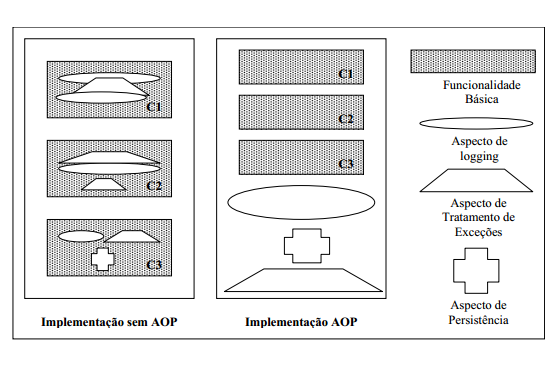
\includegraphics[scale=0.6]{figuras/funcionamentoAOP.png}
	\caption{Implementação de um sistema com e sem a utilização de aspectos.}
	\small{Fonte: \cite{steinmacher2003estudo}.}
	\label{fig:funcionamentoAOP}
\end{figure}

\section{Principais conceitos}

Para entender melhor o funcionamento de AOP, é preciso compreender seus principais conceitos. 

Os 6 principais conceitos de AOP são:

\begin{description}
\item [Aspecto] (\textit{aspect}) - pode ser definido como um interesse transversal, ou seja, interesse onde sua implementação é espalhada por diversos módulos ou componentes de um sistema.
\item [Ponto de junção] (\textit{joinpoint}) - pode ser definido basicamente como pontos bem definidos na execução de um programa.
\item [Ponto de corte] (\textit{pointcut}) - em AOP um \textit{pointcut} pode ser representado como um agrupamento de pontos de junção.
\item [Conselho] (\textit{advice}) - é a implementação de determinado interesse transversal, sendo executado quando determinado \textit{pointcut} é ativado, podendo ser executado antes (\textit{before}), em torno (\textit{around}) ou depois (\textit{after}) da execução de um ponto de junção.
\item [Introdução] (\textit{introduction}) - é quando um aspecto introduz algumas mudanças em classes, interfaces , métodos. Por exemplo, pode-se acrescentar uma variável ou método a uma classe existente  \cite{laddad2003aspectj}.
\item [Combinador] (\textit{weaver}) - é a ferramenta responsável pela combinação dos interesses centrais com os interesses transversais do sistema, ou seja,  é o momento de integração destes interesses na formação do sistema final.

\end{description}


Pode-se comparar também a complexidade de alguns conceitos de AOP com os principais conceitos de OOP:

\begin{table}[ht]
	\centering
	\caption{Comparação entre conceitos de AOP e OOP \cite{jacobson2004aspect}.}
	
	\begin{tabular}[h]{c c l}
		\hline 
		\textbf{AOP} & \textbf{OOP} \\
		\hline
		Aspecto&Classe \\
		Conselho&Método \\
		Ponto de junção&Atributo \\
		\hline
	\end{tabular}
	\label{tab:comparacaoAOPOOP}
\end{table}

\textit{Pointcut} não se encaixa em termos de complexidade em nenhum conceito de orientação a objetos, mas podemos comparar um \textit{pointcut} com um gatilho (\textit{trigger}) da linguagem SQL (\textit{Structured Query Language}) \cite{jacobson2004aspect}.

\subsection{Tipos de combinação}

Uma importante decisão de projeto que deve ser tomada, ao planejar uma ferramenta ou linguagem AOP, é o tipo de combinação que será utilizada na integração dos interesses. Existem dois tipos de combinação:

\begin{description}
\item [Estática]  consiste na modificação de \textit{bytecodes} em tempo de compilação ou de carregamento de classes, para integração dos interesses centrais e transversais. Possui um desempenho maior em relação a combinação dinâmica, por ser um processo que necessita de menos passos para ser concluído \cite{steinmacher2003estudo}.
\item [Dinâmica] a combinação é feita em tempo de execução e oferece maior flexibilidade ao programador podendo alterar, modificar e remover aspectos. Porém o desempenho do sistema é afetado, podendo causar também erros durante a execução do programa \cite{steinmacher2003estudo}. 
\end{description}

\section{Benefícios}

De forma geral pode-se dizer que todo paradigma possui seus prós e contras, sendo assim, dificilmente será encontrada uma metodologia que resolva todos os problemas da melhor maneira. Com AOP não é diferente, mas deve-se considerar sua larga escala de benefícios:

\begin{itemize}
\item Separação de interesses e Alta modularização - com AOP pode-se separar o projeto em módulos distintos, possuindo assim um acoplamento mínimo que elimina o código duplicado, fazendo com que o sistema fique muito mais fácil de entender e manter \cite{laddad2003aspectj}.
\item Fácil evolução - utilizando AOP o sistema fica muito mais flexível quando se trata da adição de novas funcionalidades, fazendo com que a resposta às exigências se tornem mais rápidas.
\item Foco na prioridade - o arquiteto do projeto pode se concentrar nos requisitos básicos atuais do sistema, os novos requisitos que abordam interesses transversais podem ser tratados facilmente com a criação de novos aspectos. AOP trabalha em harmonia com métodos ágeis, por exemplo apoia a prática YAGNI (\textit{"You aren’t gonna need it"}) \footnote{Em português significa "Você não vai precisar dele". Para saber mais sobre YAGNI consulte o Glossário.}, do \textit{Extreme Programming} (XP)\footnote{É um dos métodos ágeis mais utilizados nos dias atuais.} \cite{laddad2003aspectj}.
\item Maior reutilização de código - a chave para a reutilização de código definitiva é uma implementação flexível, com AOP é possível pois cada aspecto é implementado como um módulo distinto, se tornando adaptável a implementações equivalentes convencionais \cite{laddad2003aspectj}. 
\item Aumento na produtividade - o ciclo do projeto se torna mais rápido, a grande reutilização usada em AOP, faz com que o tempo de desenvolvimento seja reduzido, diminuindo também o tempo de implantação e o tempo de resposta às novas exigências de mercado \cite{laddad2003aspectj}. 
\item Redução de custos e aumento da qualidade - com a implementação dos interesses transversais em módulos distintos, o custo de implementação cai bastante, fazendo com que o desenvolvedor concentre-se mais nos interesses centrais, criando um produto de qualidade e com o custo reduzido.
\end{itemize}

\section{Considerações finais}

Neste capítulo foi definido os principais conceitos de AOP, que serão tomados como base para o desenvolvimento deste trabalho . Também foi possível perceber a importância em utilizar AOP como paradigma responsável pela modularização dos interesses transversais.

\chapter{Bytecode Engineering}
Neste capítulo serão abordados alguns conceitos fundamentais de \textit{bytecode}, também será definida a técnica de \textit{Bytecode Engineering}, apresentando algumas vantagens em sua utilização e ferramentas que podem ser utilizadas para aplicar esta técnica. 

\section{Fundamentos de bytecode}

Basicamente pode-se dizer que \textit{bytecode} é a linguagem intermediária entre o código fonte e o código de máquina, que faz com que os programas Java possam ser executados em múltiplas plataformas. O documento responsável pela definição de \textit{bytecode} é a Especificação da Máquina Virtual Java (\textit{Java Virtual Machine Specification})\footnote{Pode ser acessada em : http://docs.oracle.com/javase/specs/jls/se8/jls8.pdf} que descreve também os conceitos da linguagem, formato dos arquivos de classes, os requisitos da \textit{Java Virtual Machine} (JVM), entre outros \cite{kalinovsky2004covert}.

A JVM que executa sobre o sistema operacional, é responsável pelo ambiente de execução dos programas Java, sendo também a responsável pela conversão de instruções de \textit{bytecode} Java em instruções nativas de máquina \cite{stark2001java}.

\section{Definição}
\textit{Bytecode Engineering} é uma técnica normalmente utilizada para criação, manipulação e modificação de classes Java compiladas à nível de \textit{bytecode}. Muitas tecnologias  utilizam esta técnica para otimizar, ou melhorar classes já existentes.
\section {Vantagens}

Dentre as principais vantagens em utilizar \textit{Bytecode Engineering} estão:

\begin{itemize}
\item Consegue-se manipular o \textit{bytecode} sem a necessidade de recompilação, ou obtenção do código fonte original.
\item O \textit{bytecode} pode ser gerado ou instrumentado por \textit{class loader} em tempo real, enquanto as classes são carregadas em uma JVM \cite{kalinovsky2004covert}.
\item É muito mais fácil e rápido automatizar a geração de \textit{bytecode} por ser um processo mais baixo nível e também por não haver a necessidade de execução do compilador, ao contrário da geração de código fonte que possui alguns passos a mais no seu processo, e também necessita da execução do compilador \cite{kalinovsky2004covert}.
\item Instrumentar métodos, tendo como objetivo a inserção de lógica adicional, que não necessita estar nos arquivos de código fonte. Por exemplo, pode-se deixar no arquivo fonte apenas os interesses centrais do sistema, e incluir os interesses transversais utilizando \textit{Bytecode Engineering}. 
\end{itemize}

\section{Ferramentas}

Pode-se dizer que a manipulação direta de \textit{bytecode} é uma tarefa complexa, pois se trata de uma linguagem de baixo nível, e o aprendizado desta linguagem para programadores de alto nível, tende a ser muito lenta, fazendo com que seja inviável o seu aprendizado dentro do escopo de um projeto.

Pensando neste problema, foram criadas algumas bibliotecas que tornam o processo de manipulação de \textit{bytecode} mais alto nível, facilitando o seu aprendizado. As bibliotecas mais utilizadas que aplicam a técnica de \textit{Bytecode Engineering} são: \textit{Javassist}, \textit{Byte Code Engineering Library (BCEL)} e \textit{ASM}.

\subsection {Javassist}

Javassist (Assistente de Programação Java) é uma biblioteca de classes utilizada na manipulação de \textit{bytecode} em Java, permitindo que classes sejam criadas em tempo de execução e manipuladas no tempo de carregamento da JVM. A principal diferença do Javassist para outros manipuladores de \textit{bytecode}, é que Javassist possui  API no nível de código fonte e no nível de \textit{bytecode} \cite{javassist}.
\subsection {BCEL}
BCEL tem como objetivo oferecer aos usuários (desenvolvedores) uma maneira conveniente de analisar, criar, manipular arquivos de classe Java (binário). No BCEL as classes são representadas por objetos que contêm todas as suas informações (métodos, campos e instruções de \textit{bytecode}) \cite{bcel}.
\subsection {ASM}
ASM é uma estrutura de manipulação de \textit{bytecode} Java. Ela pode ser usada para gerar classes dinamicamente, diretamente na forma binária, ou modificar dinamicamente as classes em tempo de carregamento, ou seja, antes de serem carregados pela JVM. ASM oferece funcionalidades semelhantes ao BCEL, mas é muito menor e mais rápido do que essa ferramenta \cite{asmjavasource}.

\section{Considerações finais}

Pode-se perceber que a manipulação de \textit{bytecodes} não requer necessariamente conhecimentos específicos de \textit{bytecode}, além do mais existem uma variedade de \textit{frameworks} que fazem o trabalho "pesado", possibilitando a manipulação utilizando uma API de mais alto nível. Os conceitos abordados neste capítulo auxiliam o entendimento do trabalho em capítulos futuros.

\chapter{Meta programação}
Neste capítulo serão introduzidos  os principais conceitos de meta programação, falando também dos principais benefícios em aplicar esta metodologia em seus programas. Também é apresentado neste capítulo informações relevantes sobre o uso de anotações e reflexão na linguagem Java.

\section{Definição}

Meta programação por sua vez, pode ser definida como sendo um programa de computador que escreve e/ou manipula programas em tempo de execução ou compilação, fazendo com que o programa se adapte a diferentes circunstâncias, podendo controlar, monitorar ou invocar a si mesmo, visando alcançar as funcionalidades desejadas \cite{hazzard2013metaprogramming}.
\section{Benefícios}
O uso de meta programação no desenvolvimento de software pode trazer uma série de benefícios tanto para a empresa, quanto para o desenvolvedor, entre alguns dos principais benefícios estão:

\begin{itemize}
\item Simplicidade - com meta programação tem-se a possibilidade de adaptar um único bloco de código a diversas situações, sem a necessidade de geração de código, fazendo com que as classes se tornem simples e ao mesmo tempo pequenas em comparação a outros programas que não usam esta abordagem.
\item Adaptação em tempo real - pode-se fazer uma análise minuciosa do programa em tempo de execução, fazendo com que alterações no modelo de dados da aplicação sejam percebidas em tempo real, ou seja, pode-se tornar o sistema altamente configurável sem a necessidade de compilação do projeto.
\end{itemize}

\section{Principais conceitos}
Para entender melhor a meta programação, é necessário compreender seus princípios (conceitos) básicos:

\begin{description}
\item [Metalinguagem]  linguagem usada para escrever um meta programa.
\item [Meta programa ] representa um conjunto de componentes semelhantes que contém funcionalidades diferentes, que podem ser instanciados através de parametrização de modo a criar uma instância do componente específico \cite{damavsevivcius2008taxonomy}.
\item [Metadados] são dados estruturados ou codificados que descrevem as características das entidades , portando informações que visam auxiliar na identificação,  descoberta, avaliação e gestão das entidades descritas \cite{american1999task}.
\item [Reflexão] é a capacidade de um programa em observar e modificar, possivelmente, a sua estrutura e comportamento, fazendo com que a própria linguagem de programação faça o papel de metalinguagem \cite{malenfant1996tutorial}.
\end{description}

\section{Anotações em Java}
Metadados estão disponíveis na linguagem Java a partir da versão 5,  representados através de anotações (\textit{annotations}), sendo apresentada como uma das principais novidades no lançamento desta versão.
\subsection{Definição}

Uma anotação associa uma informação arbitrária ou um metadado com um elemento de um programa Java. Cada anotação tem um nome e zero ou mais membros. Cada membro tem um nome e um valor, e são
estes pares \textit{nome = valor} que carregam as informações da anotação \cite{flanagan2005java}.

Anotações são um tipo especial de interface, designado pelo caractere \textit{@} que é precedido da palavra-chave \textit{interface}. Anotações são aplicadas aos elementos do programa, ou também em outras anotações, com o intuito de fornecer informações adicionais \cite{arnold2000java}.

\subsection{Conceitos}

As anotações em Java possuem alguns conceitos importantes que devem ser compreendidos: 

\begin{description}
\item [Tipo de anotação] (\textit{annotation type}) - O nome de uma anotação, bem como os nomes, tipos e valores padrão de seus membros são definidos pelo tipo de anotação. Um tipo de anotação é essencialmente uma interface Java com algumas restrições sobre seus membros \cite{flanagan2005java}.
\item [Membro de anotação] (\textit{annotation member}) - Os membros de uma anotação são declarados em um tipo de anotação como métodos sem argumentos. O nome do método e o tipo de retorno define o nome e o
tipo do membro \cite{flanagan2005java}.
\item [Anotação marcadora] (\textit{marker annotation}) -É um tipo de anotação que não define membros, ou seja, uma anotação desse tipo traz informações simplesmente pela sua presença ou ausência \cite{flanagan2005java}.
\item [Meta-anotação] (\textit{meta-annotation}) - são anotações utilizadas para descrever o comportamento de um tipo de anotação \cite{horstmann2004core}.
\item [Alvo] (\textit{target}) - elemento do programa que será anotado.
\item [Retenção] (\textit{retention}) - é a especificação do tempo em que a informação contida na anotação é mantida. A especificação deste tempo é feita através de uma meta-anotação \cite{flanagan2005java}.
\end{description}

\subsection{Utilidades}

Utilizando anotações em Java pode-se adicionar diversas funcionalidades e recursos ao \textit{software}, sem que haja dependências entre as classes.

 Dentre as principais utilidades em usar anotações estão:

\begin{itemize}
\item Fornecer informações ao compilador - por exemplo, pode-se utilizar este recurso para detectar erros específicos em determinada parte do programa em tempo de compilação, também pode-se informar ao compilador que ignore determinados tipos de avisos, etc.
\item Processamento em tempo de compilação - normalmente utiliza-se este recurso através de ferramentas capazes de processar anotações, com o intuito de gerar código, arquivos, etc. 
\item Processamento em tempo de execução - pode-se utilizar para marcar elementos, com o objetivo de ler sua estrutura (tipo, modificadores de acesso,etc) através de reflexão em tempo de execução, fazendo com que o programa se adapte a determinadas situações.
\end{itemize}
\subsection{Exemplo}

Na figura \ref{fig:criandoAnotacao} é mostrado como criar uma anotação básica, que terá como alvo uma classe, e estará visível em tempo de execução, e também irá possuir um membro cujo tipo é uma \texttt{String}.

\begin{figure}[ht]
	\centering
	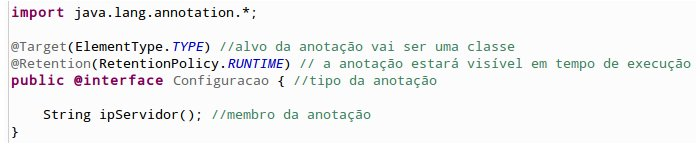
\includegraphics[scale=0.6]{figuras/criandoAnnotation.jpg}
	\caption{Criando uma anotação.}
	\small{Fonte: Autoria própria.}
	\label{fig:criandoAnotacao}
\end{figure}

Na figura \ref{fig:usandoAnotacao} é mostrado como utilizar a anotação criada na figura \ref{fig:criandoAnotacao}.

\begin{figure}[ht]
	\centering
	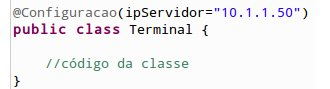
\includegraphics[scale=0.6]{figuras/usandoAnnotation.jpg}
	\caption{Utilizando uma anotação.}
	\small{Fonte: Autoria própria.}
	\label{fig:usandoAnotacao}
\end{figure}

\section{Reflexão em Java}
Na linguagem Java pode-se utilizar reflexão por meio do pacote \texttt{java.lang.reflect}, juntamente com o pacote \texttt{java.lang} que contém as classes \texttt{Class} e \texttt{Package}, e \texttt{java.lang.annotation} que faz referência à classe \texttt{Annotation}. Este conjunto de pacotes oferecem uma variedade de classes responsáveis pela leitura e modificação da estrutura de um programa em tempo de execução.


\subsection{Aplicações}

Normalmente utiliza-se reflexão para tomar alguma decisão com base na estrutura do programa, ou apenas mostrar informações sobre ela, ou seja,  utiliza-se o(s) pacote(s) de reflexão do Java para descobrir diversos tipos de informações relacionadas com a estrutura de classes, métodos, atributos e etc. Também pode-se utilizar reflexão para instanciar objetos de um tipo determinado, invocar método(s) de uma classe específica, ler anotações, entre outros.

\subsection{Funcionamento}
A reflexão em um programa Java tem inicio a partir de um objeto do tipo \texttt{Class}. Com um objeto do tipo \texttt{Class} pode-se obter sua lista completa de membros (métodos, atributos) e informações sobre eles, podendo descobrir também todos os tipos desta classe (interfaces que implementa, classes que estende), e descobrir informações sobre a própria classe, como os modificadores aplicados a ela (\texttt{public}, \texttt{protected}, \texttt{private}, etc) \cite{arnold2000java}.

\subsection{Lendo anotações}
\begin{figure}[ht]
	\centering
	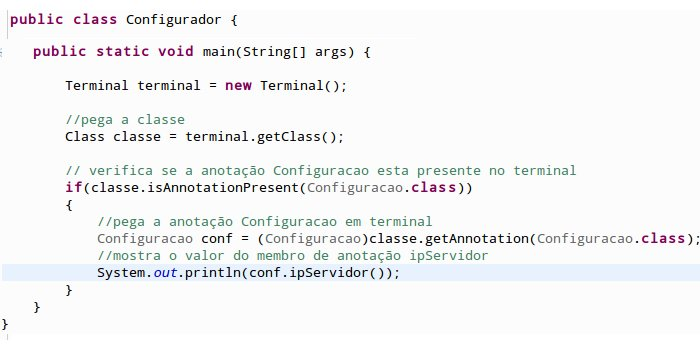
\includegraphics[scale=0.5]{figuras/lendoAnnotation.jpg}
	\caption{Lendo uma anotação.}
	\small{Fonte: Autoria própria.}
	\label{fig:lendoAnotacao}
\end{figure}
Os pacotes utilizados para reflexão possuem uma API\footnote{Visite: "http://docs.oracle.com/javase/7/docs/api/"  para saber mais sobre a API.} de fácil entendimento, e que oferecem suporte à leitura de anotações.

Na figura \ref{fig:lendoAnotacao} é mostrado como ler anotações presentes em classes, e também como ler informações presentes nos membros de uma anotação.

\section{Considerações finais}
Este capítulo apresentou os principais conceitos de Meta programação, Reflexão e Metadados. Também foi abordado neste capítulo a utilização superficial da API de reflexão e metadados da linguagem Java. 

\chapter{Tecnologias e ferramentas utilizadas}
Este capítulo apresenta  de forma clara e objetiva as tecnologias e ferramentas que serão utilizadas para o desenvolvimento deste trabalho, apresentando os motivos que fizeram com que estas ferramentas e tecnologias fossem as escolhidas para este estudo.

\section{Eclipse}

O projeto Eclipse foi inicialmente criado pela IBM no ano de 2001. No ano de 2004 foi criada a \textit{Eclipse Foundation}, uma corporação sem fins lucrativos, visando desenvolver tecnologias de código-fonte aberto com o intuito de incentivar os desenvolvedores de software a usar a tecnologia Eclipse para a construção de seus produtos e serviços de software comercial \cite{eclipsefoundation}.

O Eclipse foi escolhido como Ambiente de Desenvolvimento Integrado (\textit{Integrated Development Environment - IDE}) para a realização deste trabalho, por ser um dos mais utilizados no desenvolvimento de \textit{software} utilizando a linguagem Java, e também por oferecer diversas ferramentas que facilitam e agilizam o desenvolvimento do(s) projeto(s). Outra vantagem do Eclipse é que todas as ferramentas são oferecidas gratuitamente para uso comercial e não-comercial. 
\section{Java 7}

Java é uma linguagem de programação e plataforma computacional lançada pela primeira vez pela \textit{Sun Microsystems} em 1995.  O paradigma de programação que mais caracteriza a linguagem Java é OOP,  e uma das características que justifica a enorme compatibilidade com diversos aparelhos é a portabilidade da plataforma, que roda independentemente do sistema operacional \cite{stark2001java}. 

A proposta do trabalho justifica a escolha de Java como linguagem de programação, pois os principais objetivos envolvem um \textit{framework} AOP para linguagem Java e a utilização de técnicas de \textit{bytecode enginnering}. Será utilizado a versão 7, por ser uma versão que dispõe de diversos recursos e estabilidade alta.

\section{JavaAgent}

Agentes Java são componentes de \textit{software} que oferecem recursos de instrumentação de aplicações, recurso este que foi introduzido a partir da versão 5 do Java. No contexto dos agentes, instrumentação fornece a capacidade de re-definir o conteúdo da classe que é carregada  em tempo de execução \cite{javaagents}.

Este recurso da linguagem java será utilizado neste trabalho para interceptação das classes, com a finalidade de desenvolver o combinador de aspectos (\textit{weaver aspects}), responsável pela formação do sistema final.

\section{Javassist}

Javassist é uma biblioteca de \textit{Bytecode Enginnering} desenvolvida em cima da linguagem Java e que fornece uma API de mais alto nível em relação a outras bibliotecas do mesmo gênero \cite{javassist}.

A maioria das bibliotecas requerem um mínimo de conhecimentos de \textit{bytecode}, Javassist trabalha de forma diferente, o usuário passa para a biblioteca cadeias de caracteres no formato de código-fonte, e a própria biblioteca se encarrega de transformar esta cadeia de caracteres de código de alto nível para a linguagem de \textit{bytecode}.

A escolha da biblioteca Javassist para auxiliar na aplicação das técnicas de \textit{Bytecode enginnering} se deu devido a sua facilidade no aprendizado , além de não requerer como pré-requisito conhecimentos de \textit{bytecode}.

\section{Considerações finais}

Este capítulo apresentou de forma objetiva as principais ferramentas e tecnologias que serão utilizadas no desenvolvimento deste trabalho. Foi justificado de forma clara os motivos que contribuíram para a escolha destas ferramentas e tecnologias com o intuito de resolver o problema apresentado.

\chapter{Soluções Existentes}
Neste capítulo será abordado as características dos principais projetos relacionados existentes, e um exemplo prático de cada um deles.

\section{PostSharp}

Postsharp é um \textit{framework} para a plataforma .NET da Microsoft, responsável por encapsular os interesses transversais de sistemas.

O Postsharp possui internamente uma biblioteca de aspectos já implementados para que o desenvolvedor possa incorporar aos seus projetos  \cite{groves2013aop}.

O principal foco do Postsharp é a automação padrão dos produtos (por isso a biblioteca interna de aspectos), mas mesmo assim possui uma mega estrutura que dá suporte a criação de diversos outros tipos de aspectos \cite{groves2013aop}.

A figura \ref{fig:aspectpostsharp} mostra a implementação de um aspecto atráves do \textit{framework} Postsharp.

\begin{figure}[ht]
	\centering
	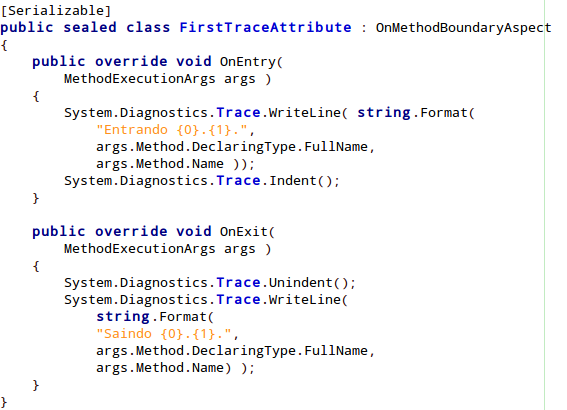
\includegraphics[scale=0.5]{figuras/ferramentas/aspectpostsharp.png}
	\caption{Exemplo de aspecto no Postsharp.}
	\label{fig:aspectpostsharp}
\end{figure}

Para criação de um aspecto através do Postsharp deve-se implementar a interface \texttt{OnMethodBoundaryAspect}, que obrigará a implementar os métodos \texttt{OnEntry} e \texttt{OnSucess}, que representam os \textit{advices before} e \textit{after}, respectivamente. 

\section{AspectJ}

O AspectJ é uma linguagem de extensão da linguagem Java, pois possui suas próprias características e palavras chaves reservadas provenientes de uma linguagem de programação. Se o AspectJ é uma extensão de Java, então todo programa que seja válido em Java, também será validado com o AspectJ \cite{laddad2003aspectj}.

Diferentemente do Postsharp o AspectJ é considerado uma linguagem de programação, pois possui sua própria sintaxe e também possui um compilador próprio que gera arquivos de \textit{bytecodes} compatíveis com a JVM \cite{laddad2003aspectj}.

A figura \ref{fig:aspectjpadrao} mostra a criação de um aspecto utilizando a sintaxe padrão da linguagem AspectJ.

\begin{figure}[ht]
	\centering
	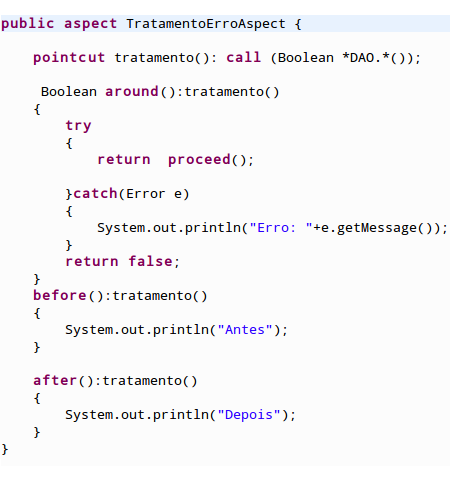
\includegraphics[scale=0.5]{figuras/aspecJ-aspecto.png}
	\caption{Exemplo de aspecto com a sintaxe padrão do AspectJ.}
	\label{fig:aspectjpadrao}
\end{figure}

A linguagem AspectJ possui palavras reservadas como \texttt{before, after, around, aspect, pointcut,call} que são interpretas pelo compilador do AspectJ durante a combinação entre classes e aspectos.

A figura \ref{fig:aspectj} mostra a criação de um aspecto utilizando o modelo de anotações  do AspectJ.

\begin{figure}[ht]
	\centering
	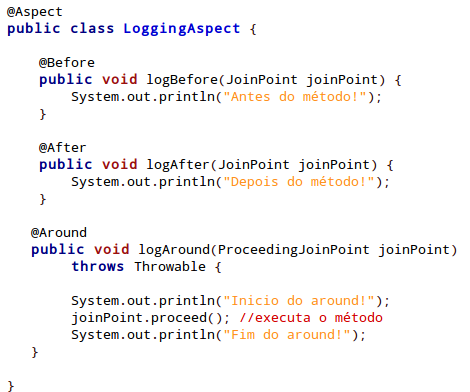
\includegraphics[scale=0.5]{figuras/ferramentas/aspectj.png}
	\caption{Exemplo de aspecto na forma de anotações no AspectJ.}
	\label{fig:aspectj}
\end{figure}

O AspectJ faz uso de uma sintaxe própria, mas também dá suporte ao uso de anotações para criação de aspectos (como mostrado na figura \ref{fig:aspectj}). A anotação responsável por informar que se trata de um aspecto é a \texttt{@Aspect}, e para informar que os métodos são \textit{advices} utilizasse das anotações \texttt{@Before, @After} e \texttt{@Around}, cuja nomenclatura representa o tipo de \textit{advice}.

\section{Considerações finais}

Este capítulo abordou as características básicas do \textit{framework} Postsharp e da linguagem AspectJ. Foi demonstrado também um exemplo prático de criação de aspectos em cada um dos projetos relacionados.

\chapter{O Framework}
\label{cap7}

Este capítulo aborda em detalhes o \textit{framework} desenvolvido, desde a parte de análise  e projeto até a parte de implementação, explicando de forma clara os caminhos percorridos durante a evolução do trabalho.

\section{Introdução}

Para a realização da análise e desenvolvimento do \textit{framework} fez-se necessário o estudo de diversos conceitos e tecnologias,  cujo embasamento teórico se encontra nos capítulos anteriores. O trabalho apresentado se concentra em torno dos seguintes conceitos: Programação Orientada à Aspectos, \textit{Bytecode Enginnering}, Meta programação (metadados e reflexão).

Para o desenvolvimento do \textit{framework} foi utilizado o Kit de Desenvolvimento Java versão 7 (\textit{Java Development Kit} - JDK), cuja versão é estável, proporcionando uma alta utilização e aceitação no mercado, fez-se uso também do Eclipse como ambiente de desenvolvimento de \textit{software}, pois possui diversas ferramentas integradas que facilitam e agilizam a programação. Foi utilizado também a biblioteca Javassist, responsável por abstrair a forma como é criado, manipulado e modificado \textit{bytecode} de classes Java em tempo de carregamento. 

Este projeto tem por intenção estudar os principais conceitos de AOP,  criando uma ferramenta para abstrair estes conceitos, de forma que facilite a aprendizagem, a aplicação prática e também sirva de base para outros estudos e pesquisas. A ferramenta projetada e desenvolvida será em forma de \textit{framework}, que terá como metodologia de uso a utilização de anotações, com o intuito de facilitar a utilização por parte do desenvolvedor e também visando um código mais limpo, concentrando as informações principais do módulo em forma de código, e as informações adicionais (conceitos de AOP) sobre as classes, métodos e atributos serão informadas em forma de metadados (anotações).
\section{Análise e projeto}

Nesta seção será apresentada a parte de análise e projeto do \textit{framework}, visando o entendimento da estrutura, arquitetura e funcionamento da ferramenta.

\subsection{Especificações do projeto}

Para cumprimento dos objetivos propostos pelo projeto, foi definido algumas especificações que devem ser cumpridas para que o projeto seja considerado apto. Entre as principais especificações estão: 
\begin{itemize}
\item A ferramenta deve ser capaz de encapsular os conceitos básicos de AOP (\textit{joinpoint, advice, aspect} e \textit{weaver}), visando uma funcionalidade genérica, que tem por objetivo separar os interesses centrais dos interesses transversais, concentrando cada interesse em seu devido módulo.

\item A ferramenta terá a capacidade de interceptação de métodos, ou seja, executar algum bloco de código antes, depois ou em volta da chamada ao método interceptado, podendo também durante esta interceptação modificar o retorno do método (caso ele retorne alguma informação). Com base nessas informações pode-se definir que os \textit{joinpoints} (pontos de junção) serão as chamadas dos métodos interceptados.

\item Os \textit{advices} (antes, depois ou em volta) serão implementados por meio de uma \texttt{interface}, que quando implementada deverá ser tratada pelo \textit{weaver} (combinador) como sendo um aspecto. Para informar ao método o tipo de aspecto e \textit{advice} que deverá ser executado na sua interceptação deve ser utilizado \textit{annotations}.

\item Para implementação do combinador deve ser utilizado técnicas de \textit{Bytecode Enginnering} para realizar modificações em classes já compiladas durante o carregamento destas classes para a Máquina Virtual do Java (JVM). O combinador será utilizado para integração dos interesses centrais com os interesses transversais durante o carregamento do sistema.
\end{itemize}
\subsection{Fluxograma}

A figura \ref{fig:fluxogramaAgent} mostra todos os processos realizados pela JVM quando é chamado um \textit{Agent} junto à chamada de um sistema.

\begin{figure}[ht]
	\centering
	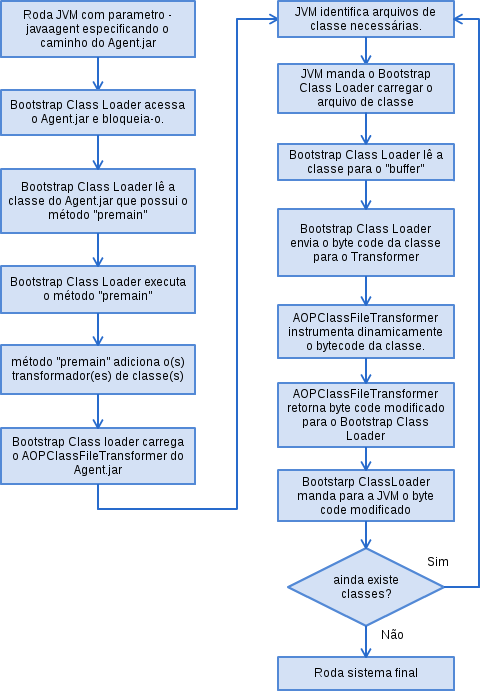
\includegraphics[scale=0.6]{diagramas/fluxograma_Agent.png}
	\caption{Fluxograma de processos da JVM na execução de um \textit{Agent} \cite{stark2001java}.}
	\label{fig:fluxogramaAgent}
\end{figure}

\subsection{Diagrama de classes}

Na figura \ref{fig:diagramaClassesAOP} é apresentado o diagrama de classes de implementação na sua forma "reduzida" utilizado como base para a implementação do \textit{framework}. Este diagrama serve para visualização do modelo de classes do sistema e seus relacionamentos, e foi construído com a ajuda da ferramenta \textit{Astah Community 6.9.0}. O diagrama de classes de implementação completo está no Apêndice \ref{apend:A}.

\begin{figure}[ht]
	\centering
	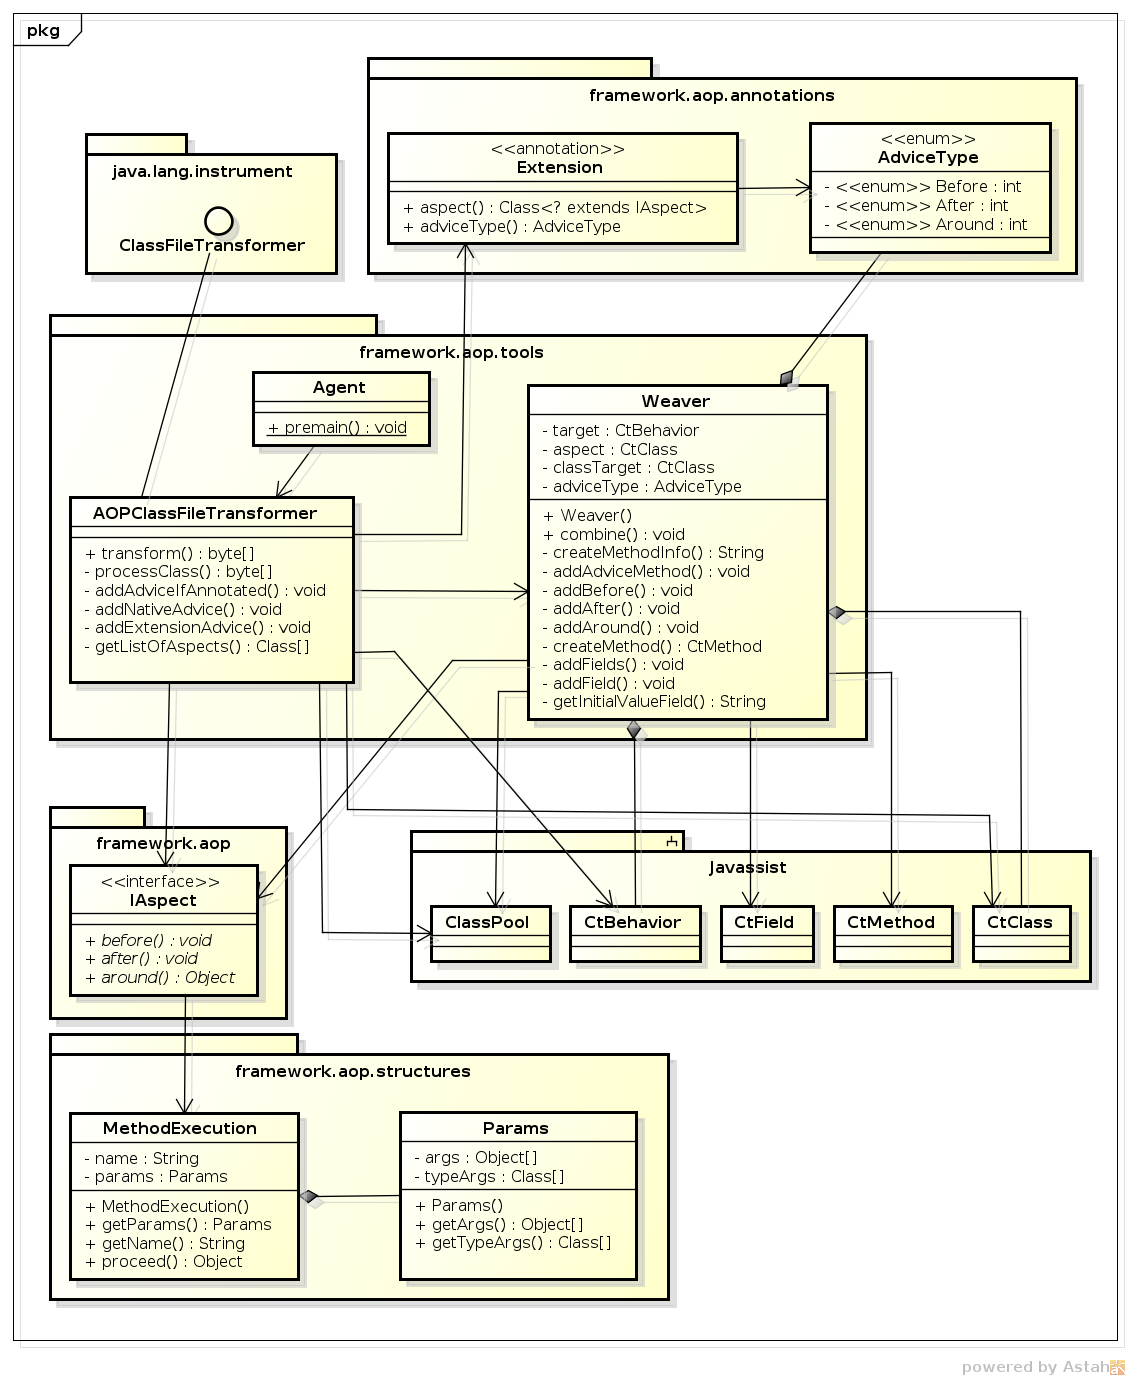
\includegraphics[scale=0.4]{diagramas/Framework_AOP.png}
	\caption{Diagrama de classes de implementação.}
	\label{fig:diagramaClassesAOP}
\end{figure}

Abaixo está a descrição de cada uma das classes apresentadas no diagrama da figura \ref{fig:diagramaClassesAOP}:

\begin{description}
\item [Agent] Esta é a classe que possui o \texttt{premain}, sendo assim é a classe principal do agente que será utilizado para interceptação das classes durante o seu carregamento para a JVM.
\item [ClassFileTransformer] Esta é uma \texttt{interface} que deve ser implementada por classes que desejam ser responsáveis pela modificação de outras classes antes do carregamento para a máquina virtual.
\item [AOPClassFileTransformer] Esta é a classe responsável por realizar e retornar para o \textit{Class Loader} (carregador de classes do Java) as classes já modificadas. Esta classe implementa a \textit{interface} ClassFileTransformer. É ela que faz a análise de quais classes vão ser combinadas, e quais as regras de combinação que devem ser consideradas para cada método. 
\item [Weaver] Esta classe representa o combinador de aspectos, ou seja, é nesta classe que são feitas as combinações de módulos OOP com módulos AOP. As informações necessárias para combinação são recebidas de \texttt{AOPClassFileTransformer}.
\item [AdviceType] É um enumerado que representa o tipo de \textit{advice}, pode ser \textit{Before} (antes), \textit{After} (depois) ou \textit{Around} (em volta). Utilizado para representar o tipo de \textit{advice} que está sendo combinado.
\item [IAspect] Esta é a \texttt{interface} que deve ser implementada pelo desenvolvedor ( usuário do \textit{framework} ) para informar que a classe será interpretada pelo modificador como sendo um aspecto.
\item [MethodExecution] Representa o método que está sendo interceptado. Possui informações sobre os parâmetros do método, e também um método auxiliar, cuja função é continuar a execução do método interceptado.
\item [Params]  Esta classe é responsável por encapsular (guardar) os tipos e valores dos parâmetros do método interceptado.
\item [ClassPool (Javassist)] Esta classe simula o \textit{Class Loader} do Java, esta classe é bastante utilizada para montar em forma de objeto as classes interceptadas.
\item [CtClass (Javassist)] Esta classe modela a estrutura de uma classe da linguagem Java, uma instância desta classe possui informações relevantes sobre ela e também métodos que navegam pela sua estrutura (métodos, atributos, construtores, etc). 
\item [CtBehavior (Javassist)] Esta classe modela de forma genérica métodos e construtores. Ela oferece métodos que são bastante utilizados para adição de código para dentro do escopo de um construtor ou método.
\item [CtMethod (Javassist)] Esta classe é parecida com \textit{CtBehavior}, porém modela apenas métodos, ou seja, possui algumas informações mais específicas sobre métodos.
\item [CtField (Javassist)] Esta classe modela um campo ou atributo de uma classe, possuindo uma gama de informações sobre eles e diversos métodos para possíveis modificações.
\end{description}

\subsection{Diagrama de sequência}

O diagrama de sequência foi utilizado para demonstrar a forma como se dá a chamada dos métodos durante o processo inicialização do \textit{Agent} até a parte de modificação (combinação de classes e aspectos) de \textit{bytecode} das classes interceptadas. Este diagrama pode ser visto na figura \ref{fig:sequenciaCombinador}.

\begin{figure}[ht]
	\centering
	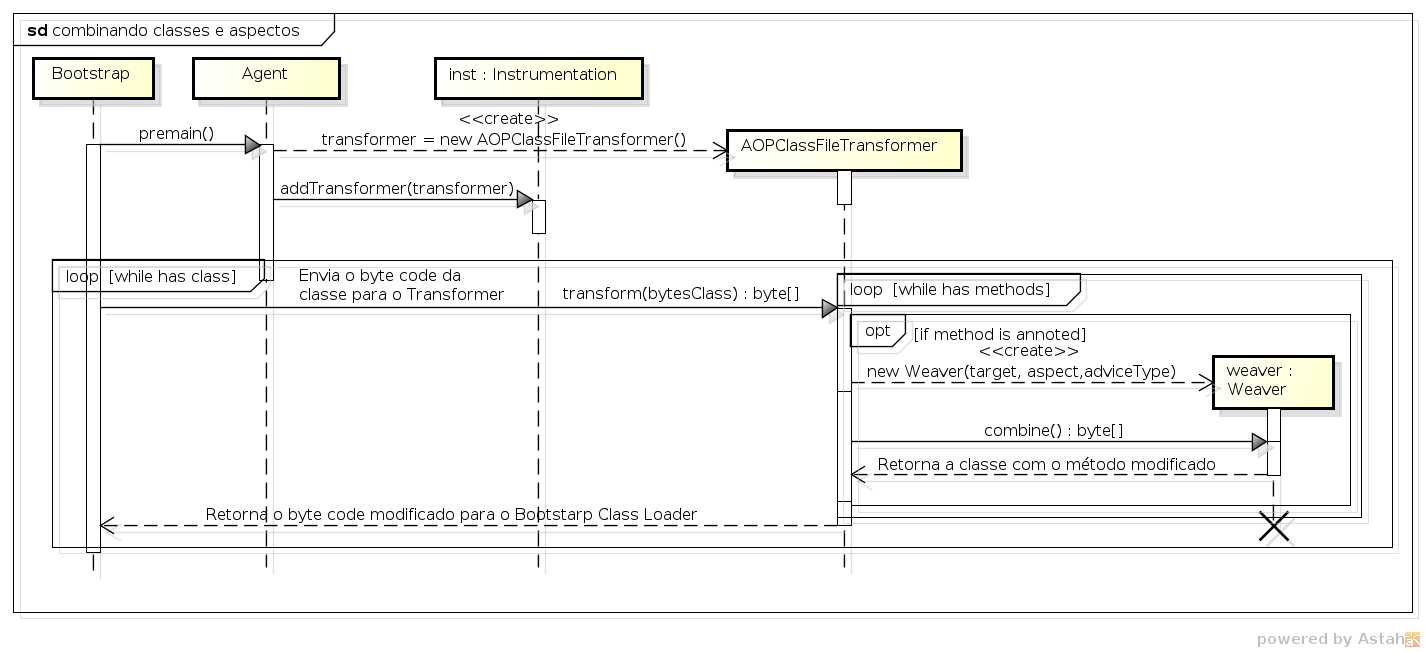
\includegraphics[scale=0.4]{diagramas/diagramaSequencia_Combinando.png}
	\caption{Diagrama de sequência.}
	\label{fig:sequenciaCombinador}
\end{figure}

O \textit{Bootstrap Class Loader} é o carregador de classes inicial, ou seja, é ele que carrega as classes e bibliotecas padrões do Java para JVM \cite{kalinovsky2004covert}. O \textit{Bootstrap Class Loader} é responsável por invocar (chamar) o método \texttt{premain} que por sua vez irá criar e adicionar o transformador de classes, neste caso \texttt{AOPClassFileTransformer}, que irá realizar a instrumentação do \textit{bytecode} das classes antes de seu carregamento para JVM.

Após criado e adicionado o transformador pelo \texttt{premain} começa o processo de instrumentação, o \textit{Bootstrap} pega o \textit{bytecode} da classe interceptada e envia através do método \texttt{transform} para o transformador realizar possíveis modificações no \textit{bytecode}.

O método \texttt{transform} por sua vez verifica todos os métodos da classe, procurando por métodos que utilizam algum tipo de aspecto de forma anotada, ou seja, métodos marcados com anotações específicas do \textit{framework}. Se alguma anotação correspondente for encontrada, então é recolhida as informações contidas nela (classe do aspecto, tipo de \textit{advice}) e enviadas para o combinador junto ao método anotado, que a partir deste momento torna-se um método alvo de interceptação.

O combinador (\texttt{Weaver}) recebe as informações necessárias para realizar a combinação da classe interceptada e do aspecto informado na anotação. Após realizada a combinação, em todos os métodos anotados da classe, é retornado então para o \textit{Bootstrap} o \textit{bytecode} da classe já modificado. O processo citado acima se dá em todas as classes que estão sendo carregadas para JVM, basicamente pode-se dizer que estas classes interceptadas são as classes do sistema que está utilizando o \textit{framework}. Maiores detalhes sobre a implementação do \textit{framework} e o seu funcionamento são encontradas na seção \ref{sec:imp}.

\section{Implementação}
\label{sec:imp}

Nesta seção será detalhada a abordagem utilizada para a implementação deste \textit{framework}. Também será discutida as características e o funcionamento geral do \textit{framework}.

\subsection{Primeiros passos}

Muitas pesquisas foram realizadas para encontrar as tecnologias capazes de suprir as necessidades do projeto, inicialmente sabia-se que deveria-se trabalhar em cima de algum \textit{framework} para aplicar as técnicas de \textit{Bytecode Enginnering} e também que deveria ser aplicada alguma técnica de interceptação ou em tempo de carregamento das classes, ou em tempo de compilação, para possíveis combinações.

Inicialmente foi realizado diversos testes utilizando a técnica de Processadores de Anotações (\textit{Annotations Processors}), que é um recurso utilizado para ler as anotações que estão visíveis em tempo de compilação. A ideia central para a utilização de Processadores de Anotações era de ler as anotações das classes em tempo de compilação, verificar se havia regras de combinação nestas anotações e posteriormente realizar a combinação. 

Esta abordagem não foi bem-sucedida pois em tempo de compilação não haveria a possibilidade de modificação das classes, pois o \textit{framework} de \textit{Bytecode Enginnering} utilizado (Javassist) só dá suporte á modificação em tempo de carregamento. Cogitou-se então 2 possíveis saídas: mudar o \textit{framework} de \textit{Bytecode Enginnering} ou mudar a forma de interceptação das classes.

Decidiu-se então mudar a técnica de interceptação de classes, pois a mudança de \textit{framework} iria atrasar o andamento do projeto, pois outros \textit{frameworks} disponíveis exigem conhecimentos específicos de \textit{bytecode}, fazendo com que se tornasse inapropriado para o escopo do projeto. Foi neste momento que decidiu-se utilizar Java Agentes como abordagem de interceptação de classes.

\subsection{Premain}

O \texttt{premain} é o método responsável pela inicialização do \textit{agent}. É dentro deste método que são adicionados o(s) transformador(es) de classes que irão realizar a interceptação. Como mostrado na figura \ref{fig:imppremain} o método \texttt{premain} do nosso \textit{agent} AOP adiciona o transformador \texttt{AOPClassFileTransformer} ao instrumentador.

\begin{figure}[ht]
	\centering
	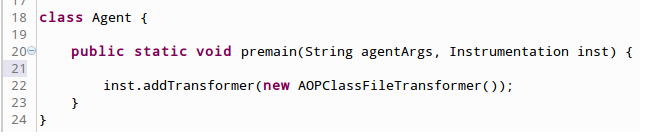
\includegraphics[scale=0.6]{figuras/implementacao/premain.png}
	\caption{Implementação do método \texttt{premain}.}
	\label{fig:imppremain}
\end{figure}

\subsubsection{Manifesto}

Existe uma configuração que deve ser feita para que o \textit{agent} saiba qual classe possui o método \texttt{premain}. Esta configuração deve ser feita em um arquivo de manifesto cujo nome deve ser \textit{Manifest.mf}, localizado dentro da pasta do projeto.  
A figura \ref{fig:manifest} mostra o conteúdo do arquivo.

\begin{figure}[ht]
	\centering
	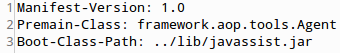
\includegraphics[scale=0.7]{figuras/implementacao/manifesto.png}
	\caption{Conteúdo do arquivo de manifesto.}
	\label{fig:manifest}
\end{figure}

A \texttt{linha 2} informa qual a classe possui o \textit{premain}, e a \texttt{linha 3} adiciona o Javassist ao caminho de classes do \textit{agent}. Este manifesto vai ser utilizado no momento da construção do arquivo \textit{.jar}.

\subsection{Transform}

Quando implementa-se a \texttt{interface ClassFileTransformer}, o desenvolvedor é obrigado a implementar o método \texttt{transform}, pois a ideia central do transformador de classes é receber e modificar o \textit{bytecode} de uma classe, sendo que o recebimento destes \textit{bytes} é feito pelo método \texttt{transform}, então obrigatoriamente ele deve estar implementado.

Na figura \ref{fig:transform} é mostrado a forma de implementação do método \texttt{transform} da classe \texttt{AOPClassFileTransformer}.

\begin{figure}[ht]
	\centering
	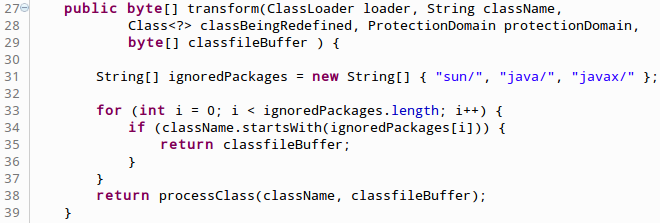
\includegraphics[scale=0.6]{figuras/implementacao/transform.png}
	\caption{Implementação do método \texttt{transform}.}
	\label{fig:transform}
\end{figure}

O \texttt{transform} armazena na variável \texttt{ignoredPackages} os pacotes que devem ser ignorados, ou seja, as classes que pertencem aos pacotes listados (classes padrão do Java) vão ser ignoradas pelo transformador, retornando para o \textit{Bootstrap Class Loader} o seu \textit{bytecode} original. Se a classe interceptada não for uma classe padrão do Java, então ela será processada pelo método \texttt{processClass}, cuja implementação está na figura \ref{fig:processClass}.

\begin{figure}[ht]
	\centering
	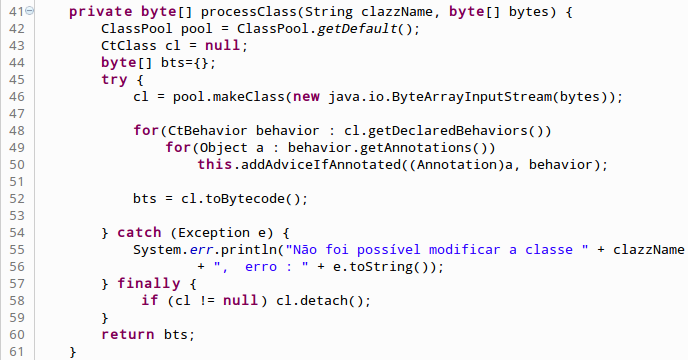
\includegraphics[scale=0.5]{figuras/implementacao/processClass.png}
	\caption{Implementação do método \texttt{processClass}.}
	\label{fig:processClass}
\end{figure}

Através do \textit{bytecode} da classe que foi recebido por parâmetro, o método \texttt{processClass}, monta a classe recebida em um objeto do tipo \texttt{CtClass}. Objetos do tipo \texttt{CtClass} possuem informações sobre toda a estrutura de uma classe, sendo assim percorre-se todos os métodos existentes na classe  em busca de métodos anotados. Para cada anotação existente em um método é invocada uma chamada ao método \texttt{addAdviceIfAnnotated}. A implementação deste método pode ser vista na figura \ref{fig:addadviceifannotated}.

\begin{figure}[ht]
	\centering
	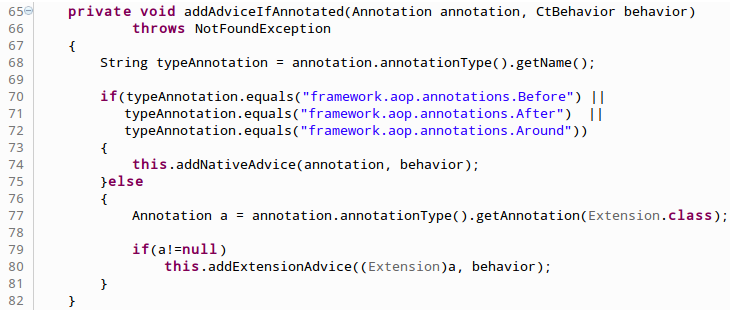
\includegraphics[scale=0.6]{figuras/implementacao/addadviceifannotated.png}
	\caption{Implementação do método \texttt{addAdviceIfAnnotated}.}
	\label{fig:addadviceifannotated}
\end{figure}

O método \texttt{addAdviceIfAnnotated} é responsável por verificar se a anotação presente no método é uma anotação suportada pelo \textit{framework}, se for repassa a responsabilidade para o método mais apropriado para tratar o modelo de anotação utilizado.

Se a anotação for nativa é chamado o método \texttt{addNativeAdvice}, caso contrário ela será uma anotação de extensão, cujo método chamado será \texttt{addExtensionAdvice}. A implementação de \texttt{addNativeAdvice} e \texttt{addExtensionAdvice}, são mostradas nas figuras \ref{fig:addnativeadvice} e \ref{fig:addextensionadvice}, respectivamente.

\begin{figure}[ht]
	\centering
	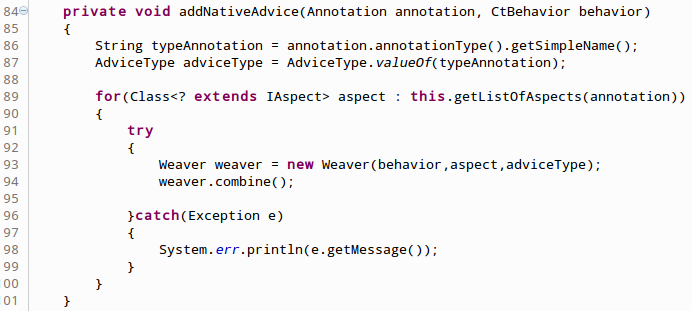
\includegraphics[scale=0.5]{figuras/implementacao/addnativeadvice.png}
	\caption{Implementação do método \texttt{addNativeAdvice}.}
	\label{fig:addnativeadvice}
\end{figure}

\begin{figure}[ht]
	\centering
	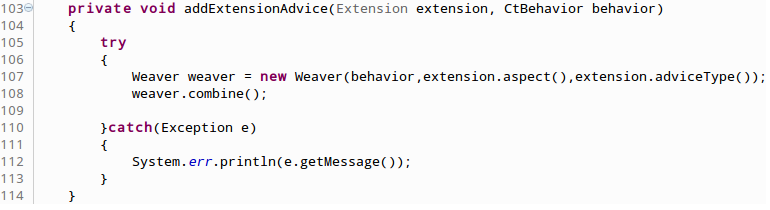
\includegraphics[scale=0.5]{figuras/implementacao/addextensionadvice.png}
	\caption{Implementação do método \texttt{addExtensionAdvice}.}
	\label{fig:addextensionadvice}
\end{figure}

O foco dos métodos representados nas figuras \ref{fig:addnativeadvice} e \ref{fig:addextensionadvice} se resume em recolher as informações contidas nas anotações (anotações nativas e de extensão), e posteriormente mandar as informações recolhidas para o combinador (\textit{Weaver}). As informações que o combinador precisa receber são: método interceptado, aspecto e tipo de \textit{advice}. 

A classe \texttt{Weaver}, responsável pela combinação será detalhada na seção  \ref{combinacao}, neste mesmo capítulo.

\subsubsection{Anotações nativas}

As anotações nativas são anotações (\textit{annotations}) utilizadas por padrão pelo \textit{framework} para marcar o tipo de \textit{advice} utilizado e a qual aspecto este \textit{advice} pertence. 

O \textit{framework} possui 3 anotações nativas: \texttt{@Before, @After, @Around}. Sendo que todas elas recebem um parâmetro que representa o aspecto que possui o \textit{advice}, da seguinte forma: \texttt{NomeDoAspecto.class}.

\subsubsection{Anotações de extensão}

As anotações de extensão foram criadas para oferecer ao desenvolvedor uma forma de estender as anotações nativas, dando-lhes a oportunidade de criar uma API mais simples e uma melhor descrição do interesse transversal implementado como aspecto.

Por exemplo se é criado um aspecto para modularizar a lógica de \textit{cache}, sendo que esta lógica envolve apenas o \textit{advice around}. De forma nativa a anotação utilizada para marcar a utilização de \textit{cache} em um método seria a seguinte: \texttt{@Around(Cache.class)}. Por outro lado se o desenvolvedor criar uma anotação que estende a anotação \texttt{@Around}, ele pode conseguir o seguinte resultado na utilização: \texttt{@Cache}, obtendo uma leitura mais limpa e uma API personalizada. A criação e a utilização de anotações de extensão será demonstrada no capítulo \ref{estudodecaso} referente ao estudo de caso.

\subsection{Combinador}
\label{combinacao}

A utilização de AOP junto à OOP, resulta em um sistema altamente modularizado, organizado e semanticamente correto à nível de código-fonte. Mas a integração entre os dois paradigmas deve ser feita em algum momento para que haja uma comunicação entre os módulos. Esta comunicação é feita à nível de \textit{bytecode}, sendo assim o desenvolvedor não visualiza esta comunicação. A única forma de relacionamento entre os dois paradigmas à nível de código-fonte é através de anotações, tornando muito mais simples o entendimento e a aplicação de relacionamentos entre módulos. Desta forma os módulos se tornam completamente desacoplados, ou seja, um módulo não depende do outro diretamente.

A responsável por realizar essas combinações à nível de \textit{bytecode} é a classe \texttt{Weaver}. Esta classe faz uso das técnicas de \textit{Bytecode Enginnering} através da utilização do \textit{framework} Javassist.

\begin{figure}[ht]
	\centering
	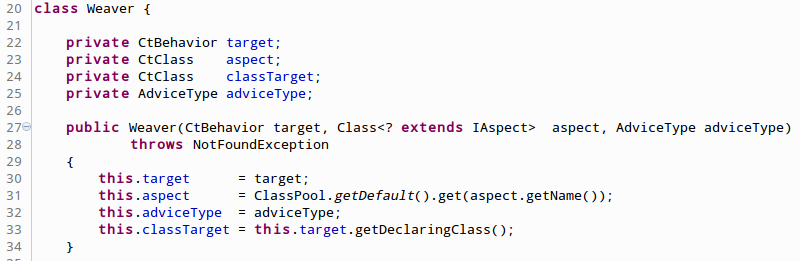
\includegraphics[scale=0.5]{figuras/implementacao/weaver.png}
	\caption{Atributos e construtor da classe \texttt{Weaver}.}
	\label{fig:weaver}
\end{figure}

A classe \texttt{Weaver} possui quatro atributos, como pode ser visto na figura \ref{fig:weaver}:

\begin{description}
\item [target] Este atributo irá armazenar o método alvo de interceptação e a sua estrutura, para possíveis modificações.
\item [aspect] Este atributo armazena a classe que representa o aspecto utilizado pelo método alvo. Este atributo é uma das chaves para a combinação.
\item [classTarget] Este atributo armazena a classe que possui o método alvo, ou seja, alterações realizadas fora do método alvo serão feitas através deste objeto.
\item [adviceType] Este atributo é utilizado para saber qual o tipo de \textit{advice} do aspecto está sendo utilizado. Este atributo será fundamental para o recolhimento de informações do aspecto.
\end{description}

Para construir um novo combinador é preciso informar algumas regras básicas de combinação. Estas regras são informadas através do construtor que recebe uma instância do método alvo, o \textit{.class} do aspecto (\texttt{nomeDoAspecto.class}), e o tipo de \textit{advice} da combinação.

A classe estática \texttt{ClassPool} é um canal intermediário de comunicação entre o \textit{Class Loader} e o \textit{framework}. No construtor é necessário acessar o \textit{Class Loader} através do \texttt{ClassPool} para conseguir uma instância de \texttt{CtClass} para acessar as estrutura do aspecto.

Após a execução do construtor da classe \texttt{Weaver}, ou seja, após a criação do combinador, é executado o método \texttt{combine}, que inicia o processo de combinação. A implementação do método \texttt{combine} é mostrada na figura \ref{fig:combine}.

\begin{figure}[ht]
	\centering
	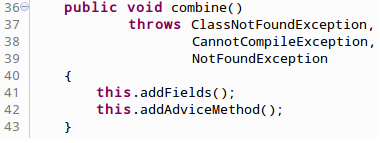
\includegraphics[scale=0.6]{figuras/implementacao/combine.png}
	\caption{Implementação do método \texttt{combine}.}
	\label{fig:combine}
\end{figure}

A implementação do método \texttt{combine} é bem simples, ele apenas chama outros dois métodos. O \texttt{addFields} e seus "sub-métodos" encapsulam toda a lógica de adição de novos campos na classe alvo, ou seja, todos campos existentes no aspecto e que não estão na classe alvo são copiados. Já o método \texttt{addAdviceMethod} e seus "sub-métodos" encapsulam a lógica de combinação do método interceptado com o seu \textit{advice} correspondente. 

Nas próximas subseções serão abordados os detalhes de implementação dos dois métodos citados acima.

\subsubsection{AddFields}

Para iniciar realmente o processo de combinação, deve-se começar copiando os campos existentes no aspecto para a classe alvo, caso esses campos ainda não existam. Este processo inicia pelo método \texttt{addFields}, cuja implementação está na figura \ref{fig:addfields}.

\begin{figure}[ht]
	\centering
	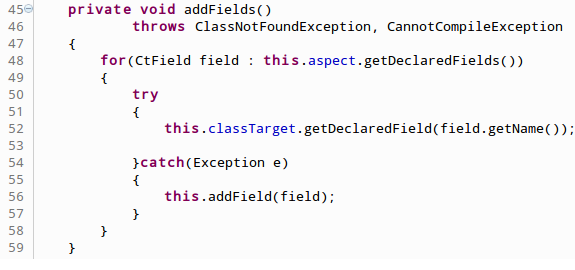
\includegraphics[scale=0.6]{figuras/implementacao/addfields.png}
	\caption{Implementação do método \texttt{addFields}.}
	\label{fig:addfields}
\end{figure}

O método \texttt{addFields} verifica se cada campo existente no aspecto, existe na classe alvo, caso não exista é chamado o método \texttt{addField} para realizar a cópia deste campo para a classe alvo. Pode-se notar que a API do Javassist não oferece um método para verificar se determinado campo existe, mas ela lança uma exceção quando tenta-se acessar algum membro inexistente. Pensando desta forma fez-se o uso de um bloco \texttt{try-catch} para verificar se o campo já existe, se a execução do método cair no bloco \texttt{catch} significa que uma exceção foi capturada e o campo não existe, providenciando então a sua cópia pelo método \texttt{addField}. O método \texttt{addField} e sua implementação pode ser vista na figura \ref{fig:addfield}.

\begin{figure}[ht]
	\centering
	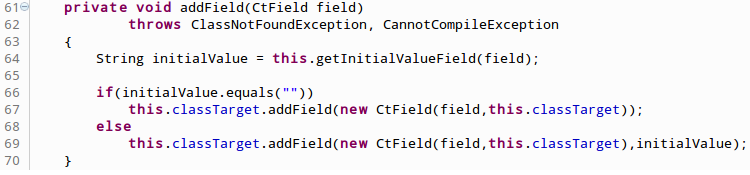
\includegraphics[scale=0.5]{figuras/implementacao/addfield.png}
	\caption{Implementação do método \texttt{addField}.}
	\label{fig:addfield}
\end{figure}

O método \texttt{addField} é responsável por adicionar o campo à classe alvo. Primeiramente é obtido o valor inicial do campo através do método \texttt{getInitialValueField}, caso não tenha sido declarado nenhum valor inicial é retornado uma \texttt{String} vazia. Após obter, ou não o valor inicial do campo, é utilizado o método \texttt{addField} da classe alvo para realizar a adição do campo, este método recebe uma nova instância de \textit{CtField} que recebe o campo a ser copiado, e a classe que receberá este campo.

Na figura \ref{fig:getinitialvaluefield} é mostrado a implementação de \texttt{getInitialValueField}.

\begin{figure}[ht]
	\centering
	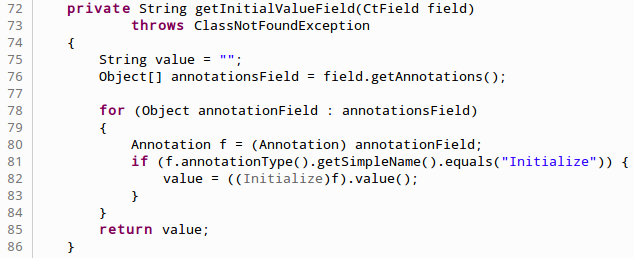
\includegraphics[scale=0.6]{figuras/implementacao/getinitialvaluefield.png}
	\caption{Implementação do método \texttt{getInitialValueField}.}
	\label{fig:getinitialvaluefield}
\end{figure}

No aspecto o valor inicial de um campo pode ser informado através da utilização da anotação \texttt{@Initialize("valor")} antes do campo a ser inicializado, esta anotação foi criada pois através do Javassist não é possível pegar o valor de um campo. Desta forma se um campo for inicializado no aspecto através do operador \texttt{=}, esta inicialização não estará visível na combinação, por exemplo: \texttt{private int idade = 18}. Sendo assim a inicialização correta do campo seria: \texttt{@Initialize("18") private int idade}.

Basicamente então para o método \texttt{getInitialValueField} pegar o valor inicial do campo, basta ler as anotações existentes no campo e verificar se ele possui a anotação \texttt{@Initialize}, se possuir retorna o valor inicial, caso contrário retorna uma \texttt{String} vazia.

\subsubsection{AddAdviceMethod}

Após a cópia dos campos para a classe alvo, é necessário realizar a integração entre o \textit{advice} e o método interceptado. É dada a partida para essa integração através da chamada ao método \texttt{addAdviceMethod}, cuja responsabilidade é fazer uma cópia do \textit{advice} e repassar esta cópia para o método correspondente ao tipo de \textit{advice}. Os métodos que combinam cada tipo de \textit{advice} são: \texttt{addBefore}, \texttt{addAfter} e \texttt{AddAround}. Na figura \ref{fig:addadvicemethod} é mostrado a implementação do método \texttt{addAdviceMethod}.

\begin{figure}[ht]
	\centering
	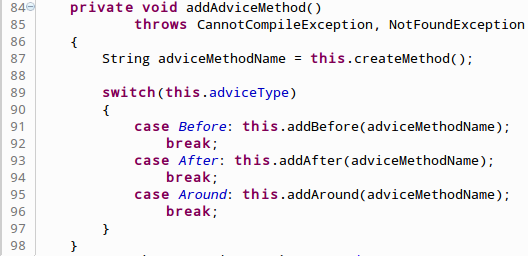
\includegraphics[scale=0.5]{figuras/implementacao/addadvicemethod.png}
	\caption{Implementação do método \texttt{addAdviceMethod}.}
	\label{fig:addadvicemethod}
\end{figure}

O método \texttt{createMethod} é responsável por fazer a cópia do \textit{advice} para a classe alvo, e também por adicionar configurações ao método caso seja necessário. Este método faz a verificação se a classe alvo já não possui um método correspondente ao \textit{advice}, caso não possua é feita a cópia. Se o \textit{advice} utilizado for \textit{before} ou \textit{after} é adicionado um bloco \texttt{try/catch} ao \textit{advice} copiado, para tratar possíveis exceções lançadas por estes \textit{advices}. Após estes procedimentos a cópia é realmente adicionada à classe alvo. A figura \ref{fig:createmethod} mostra a implementação de \texttt{createMethod}.

\begin{figure}[ht]
	\centering
	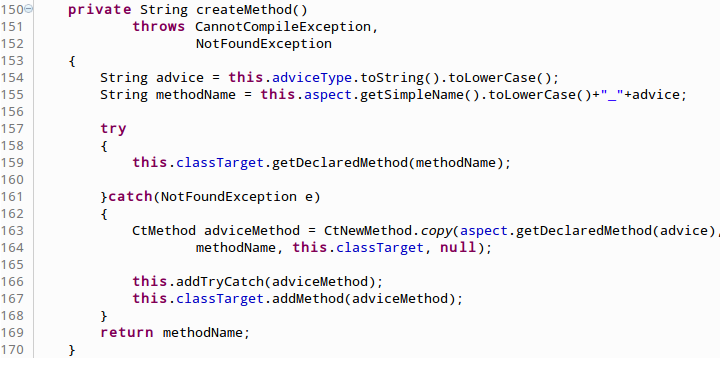
\includegraphics[scale=0.5]{figuras/implementacao/createmethod.png}
	\caption{Implementação do método \texttt{createMethod}.}
	\label{fig:createmethod}
\end{figure}

Para realizar a combinação do método com um \textit{advice} do tipo \textit{before} é utilizado o método \texttt{addBefore}. O nome do método copiado recebido por parâmetro é formado da seguinte maneira: \texttt{aspecto\$advice}. Para adicionar uma chamada à cópia do \textit{advice} antes da execução do método interceptado é necessário utilizar o método \texttt{insertBefore} presente na classe \texttt{CtMethod} do Javassist. A chamada para o método \texttt{insertBefore} deve ser realizada pela instância do método interceptado. Na figura \ref{fig:addbefore} está a implementação do método \texttt{addBefore} da classe \texttt{Weaver}.

\begin{figure}[ht]
	\centering
	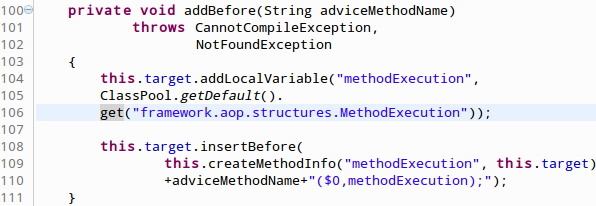
\includegraphics[scale=0.5]{figuras/implementacao/addbefore.png}
	\caption{Implementação do método \texttt{addBefore}.}
	\label{fig:addbefore}
\end{figure}

Adicionou-se uma variável local que chama-se \texttt{methodExecution} e é do tipo \texttt{MethodExecution} ao método alvo, esta variável é utilizada para armazenar as informações do método (valor dos parâmetros, tipo dos parâmetros, etc). Para formar a cadeia de caracteres que representa a instanciação da variável é utilizado o método \texttt{createMethodInfo} (na figura \ref{fig:createmethodinfo} encontra-se a implementação deste método). O método \texttt{insertBefore} recebe como parâmetro uma \texttt{String} que representa o código que deve ser adicionado antes da execução do método alvo, esta \texttt{String} é formada pela instanciação da variável local e pela chamada á cópia do \textit{advice}.  Para realizar a chamada ao \textit{advice} que foi copiado para a classe alvo, deve-se ter dois parâmetros em mãos, o primeiro representado por (\textit{\$0}) representa a instância real da classe que possui o método, e o segundo a instância de \texttt{MethodExecution}, explicado anteriormente.


\begin{figure}[ht]
	\centering
	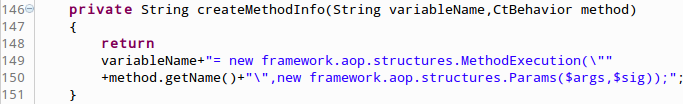
\includegraphics[scale=0.5]{figuras/implementacao/createmethodinfo.png}
	\caption{Implementação do método \texttt{createMethodInfo}.}
	\label{fig:createmethodinfo}
\end{figure}

Pode-se notar que para instanciar a classe \texttt{Params} na \texttt{linha 150} da figura \ref{fig:createmethodinfo} é passado dois parâmetros, o primeiro (\textit{\$args}) representa um objeto do tipo \texttt{Objeto[]} que possui os valores dos parâmetros e o segundo (\textit{\$sig}) é do tipo \texttt{Class[]} que possui os tipos de cada parâmetro. Esta sintaxe utilizada em forma de \texttt{String} é traduzida para \textit{bytecode} pelo Javassist.
 
O método \texttt{addAfter} foi implementado praticamente da mesma forma que o método \texttt{addBefore}, sendo que a única diferença é que \texttt{addAfter} faz a utilização do método \texttt{insertAfter} para adicionar código depois, e o \texttt{addBefore} utiliza o método \texttt{insertBefore} para adicionar antes. A implementação de \texttt{addAfter} pode ser vista na figura \ref{fig:addafter}.
 
 
\begin{figure}[ht]
	\centering
	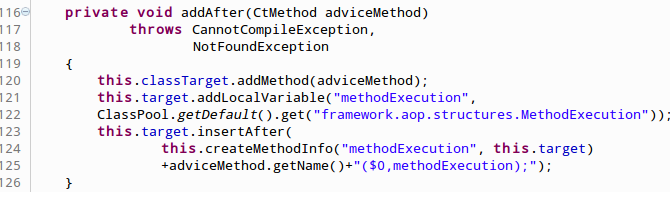
\includegraphics[scale=0.6]{figuras/implementacao/addafter.png}
	\caption{Implementação do método \texttt{addAfter}.}
	\label{fig:addafter}
\end{figure}

O \textit{advice} do tipo \textit{around} se resume em envolver a execução de um método com trechos de código, ou seja, nada mais é do que adicionar código antes e depois da chamada a um método. O tipo \textit{around}
é um pouco mais complexo que \textit{before} e \textit{after}, e também o mais utilizado no encapsulamento de interesses transversais mais complexos.  

O método da classe \texttt{Weaver} responsável por realizar a combinação do método interceptado com o \textit{advice around} é o método \texttt{addAround}, e a sua implementação se encontra na figura \ref{fig:addaround}.

\begin{figure}[ht]
	\centering
	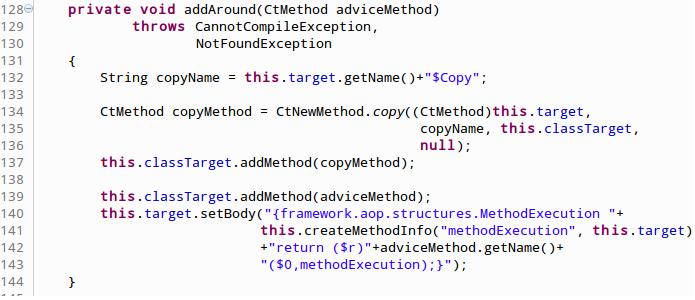
\includegraphics[scale=0.5]{figuras/implementacao/addaround.png}
	\caption{Implementação do método \texttt{addAround}.}
	\label{fig:addaround}
\end{figure}

A implementação de \texttt{addAround} segue o mesmo modelo de implementação de \texttt{addBefore} e \texttt{addAfter}, porém desenvolvida de forma diferente. Primeiramente é preciso realizar uma cópia do método alvo, para manter a implementação intacta, o nome do método copiado terá a seguinte forma: \texttt{nomeOriginalMétodo\$Copy}. Tendo a cópia do método, deve-se então reescrever o corpo do método original, para isso utiliza-se o método \texttt{setBody} disponível em instâncias de \texttt{CtMethod} do Javassist. Para adicionar variáveis locais ao corpo do método não é utilizado o método \texttt{addLocalVariable}, sendo assim foi utilizado o formato de \textit{String} para adicionar a variável \texttt{methodExecution}. É adicionado também ao corpo do método a chamada ao \textit{advice} copiado.

Para informar ao \textit{advice around} o momento que deve ser executado o método original dentro do seu escopo, deve-se fazer a utilização do método \texttt{proceed} presente na instância da classe \texttt{MethodExecution} recebida por parâmetro. Na figura \ref{fig:exemploproceed} um exemplo da utilização do \texttt{proceed} em um \textit{advice around}.

\begin{figure}[ht]
	\centering
	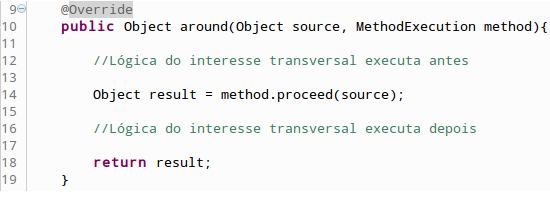
\includegraphics[scale=0.5]{figuras/implementacao/exemplo_proceed.png}
	\caption{Exemplo de implementação do \textit{advice around}.}
	\label{fig:exemploproceed}
\end{figure}

O método \texttt{proceed} faz o uso de reflexão para invocar uma chamada à copia do método original feita no \texttt{addAround}, esta chamada é feita pelo objeto \texttt{source}, que seria uma instância da classe alvo, ou seja, a classe que recebeu a cópia do método. A implementação de \texttt{proceed} realizada na classe \texttt{MethodExecution}, pode ser vista na figura \ref{fig:proceed}. 

\begin{figure}[ht]
	\centering
	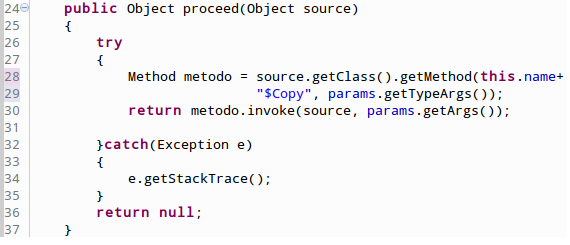
\includegraphics[scale=0.5]{figuras/implementacao/proceed.png}
	\caption{Implementação do método \texttt{proceed}.}
	\label{fig:proceed}
\end{figure}

\section{Considerações finais}

Este capítulo abordou as características do projeto e todos os seus detalhes de implementação, com o intuito de oferecer uma base teórica e prática para estudos sobre AOP. No próximo capítulo será utilizado os conhecimentos aqui adquiridos para o desenvolvimento de um estudo de caso.

\chapter{Estudo de caso - Instrumentação}
\label{estudodecaso}

Neste capítulo será desenvolvido um estudo de caso para demonstrar as funcionalidades do \textit{framework}. Neste capítulo será abordado a parte de análise e desenvolvimento do estudo de caso, e também detalhes sobre a combinação dos aspectos com as classes.

\section{Introdução}

Nos dias atuais a quantidade de produtos, serviços e ferramentas desenvolvidas para resolução de um problema é imensa, devido o aumento das necessidades em geral. No mundo do desenvolvimento de \textit{software} não é diferente, sistemas, aplicativos e ferramentas também são desenvolvidas visando na maioria das vezes a resolução de um problema, ou facilitar (automatizar) a execução de uma tarefa. 

Pensando nisso são desenvolvidos casos de testes e/ou estudos de casos para demonstrar a eficiência e a capacidade de resolução do problema proposto, levando em conta a visão do cliente (usuário). Para demonstrar a capacidade do \textit{framework} de encapsular interesses transversais e a facilidade adquirida na sua utilização, será desenvolvido um estudo de caso para comprovar de forma prática os conceitos apresentados.

\section{O problema}

Um sistema hipotético, é formado por diversos módulos, sendo que cada módulo tem uma responsabilidade específica. Levando em conta que o carregamento destes módulos se dá durante a inicialização do sistema, deve-se calcular o tempo de carregamento de cada módulo, e também o tempo total de carregamento do sistema, armazenando estas informações em um arquivo de \textit{log}\footnote{Para saber mais sobre \textit{log} consulte o Glossário ao final deste texto.}. A solução deste problema deve se dar de forma que código referente ao cálculo do tempo de execução não esteja entrelaçado e/ou espalhado pelos módulos do sistema, fazendo com que o sistema e seus módulos sejam totalmente independentes em relação ao gerenciamento de tempo de cada módulo.

\subsection{Instrumentação}

Instrumentação é o nome dado à inserção de código adicional ao sistema, visando analisar e avaliar diversas medidas de desempenho durante a execução de um programa \cite{cabral2005instrumentaccao} . 

A medida de desempenho aqui utilizada será o cálculo do tempo de execução de um método, com o intuito de avaliar o tempo de carregamento do sistema, realizando uma análise nos métodos envolvidos nesta tarefa.

\subsection{Solução}

Para resolução do problema vai ser utilizado o \textit{framework} desenvolvido para criação dos aspectos, que também será responsável pela integração entre as classes referentes ao sistema e o aspecto referente ao cálculo de execução dos métodos.

A única forma de comunicação entre a classe e o aspecto será uma anotação (nativa ou de extensão), cuja principal finalidade é marcar quais métodos devem ser interceptados, de que forma, e o que deve ser executado durante esta interceptação.

\section{Análise}

Para descrever a parte de análise do estudo de caso foi desenvolvido um diagrama de classes de implementação, que mostra toda a estrutura e o relacionamento entre as partes envolvidas no projeto.

A figura \ref{fig:estudodiagrama} mostra o diagrama de classes do estudo de caso, que serviu de base para a implementação.


\begin{figure}[ht]
	\centering
	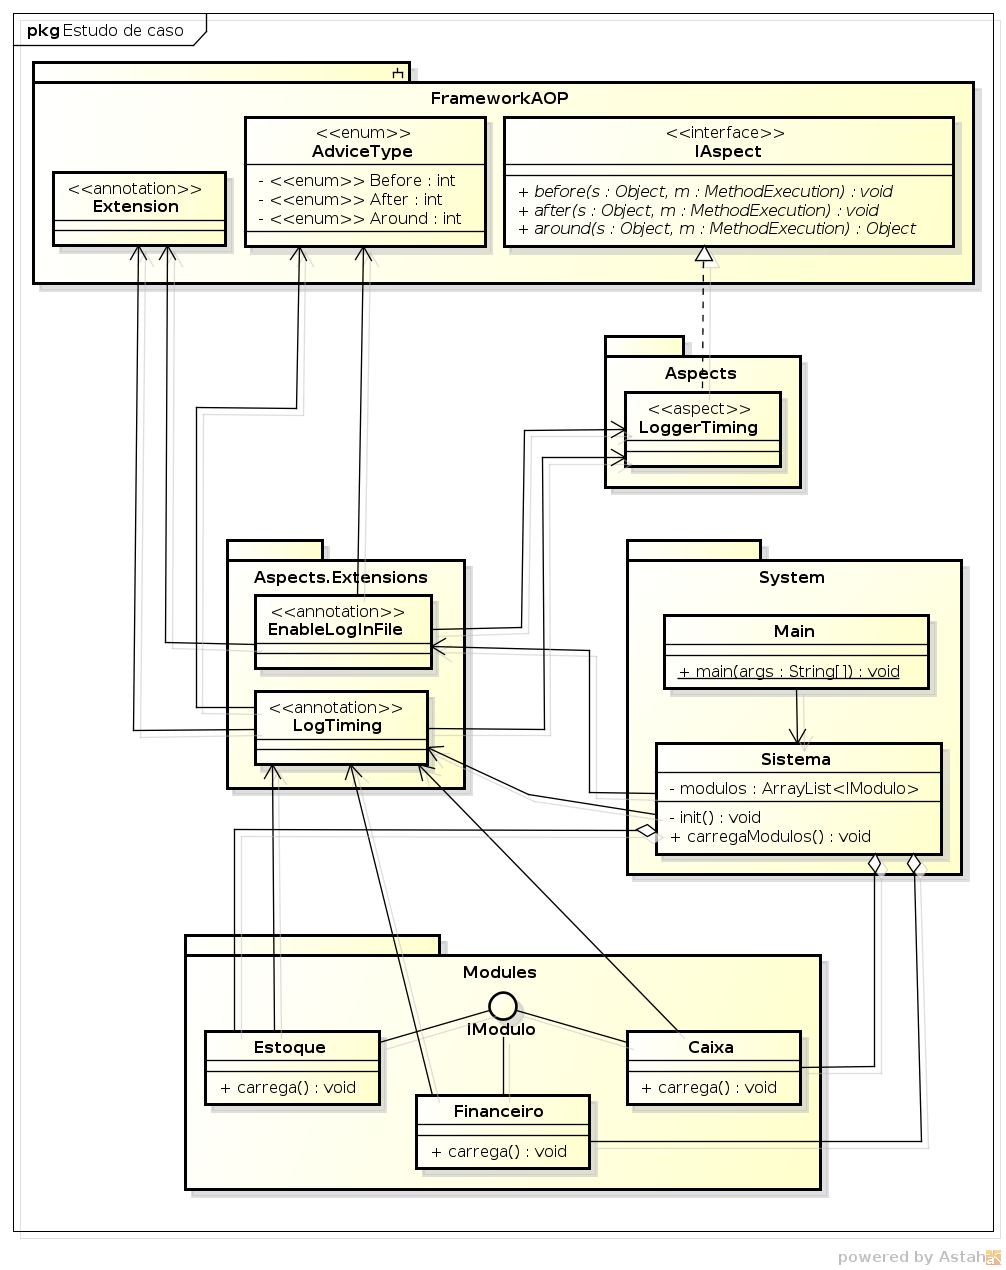
\includegraphics[scale=0.4]{diagramas/estudoCaso.png}
	\caption{Diagrama de classes do estudo de caso.}
	\label{fig:estudodiagrama}
\end{figure}

As classes referentes ao \textit{framework} presentes no diagrama da figura \ref{fig:estudodiagrama} não serão descritas neste capítulo porque já foram descritas no capítulo \ref{cap7}. Abaixo está a descrição das outras classes presentes no diagrama.

\begin{description}

\item [Main] Esta classe é a responsável por iniciar o sistema e suas configurações.
\item [Sistema] Esta classe representa o sistema hipoteticamente. Esta classe possui os módulos do estudo.
\item [IModulo] Interface que deve ser implementada por todos os módulos. Esta interface obriga a implementação.
\item [Estoque, Caixa, Financeiro] Classes hipotéticas que representam os módulos do sistema.
\item [LoggerTiming] Este é o aspecto que irá encapsular a lógica responsável por calcular o tempo de execução dos métodos, e também a lógica que ativa o armazenamento das informações obtidas através de instrumentação em um arquivo de \textit{log}.
\item [EnableLogInFile] Esta anotação é responsável por marcar o método que irá ativar o armazenamento em \textit{log} antes de sua execução.
\item[LogTiming] Esta anotação é utilizada para informar que o método anotado terá o seu tempo de execução calculado.
\end{description}

\section{Implementação}

Para demonstrar as funcionalidades do \textit{framework} procurou-se desenvolver um estudo de caso simples, mas que cumpra o esperado. Pensando desta forma, decidiu-se focar a parte implementação não no sistema que representa os interesses centrais, mas sim nos aspectos que representam os interesses transversais de um sistema. Sendo assim, não foi implementando um sistema funcional, mas sim uma estrutura que representasse este sistema.

\subsection{Criação de um aspecto}

Para criação de um aspecto utilizando o \textit{framework} deve-se implementar a interface \texttt{IAspect} presente no pacote \texttt{framework.aop} detalhado no diagrama de classes da figura \ref{fig:diagramaClassesAOP}. A implementação do aspecto \texttt{LoggerTiming} está representada nas figuras \ref{fig:loggeraspectaround} e \ref{fig:loggeraspectbefore}.

\begin{figure}[ht]
	\centering
	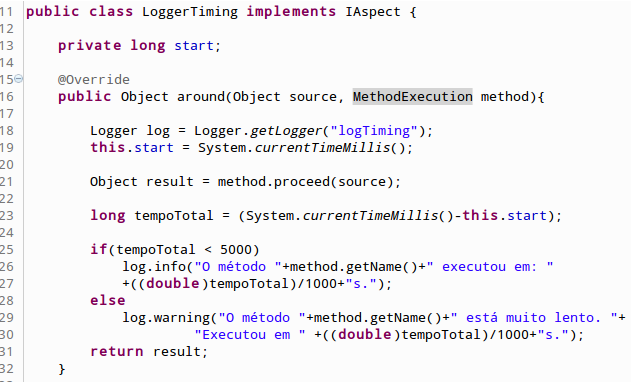
\includegraphics[scale=0.6]{figuras/estudo/loggertimingaround.png}
	\caption{Implementação do \textit{advice} \texttt{around} do aspecto \texttt{LoggerTiming}.}
	\label{fig:loggeraspectaround}
\end{figure}
O \textit{advice} \texttt{around} do aspecto \texttt{LoggerTiming} possui a função de calcular o tempo de execução de um método, de forma que todo o código necessário para execução desta função está encapsulado neste \textit{advice}. Pode-se notar que na linha \texttt{21} é onde ocorre a execução do método interceptado.

Caso o método executado tenha sua execução realizada em um tempo maior que 5 segundos, é mostrado no \textit{log} um aviso, caso contrário é mostrado um \textit{log} de informação com o tempo de execução.

\begin{figure}[ht]
	\centering
	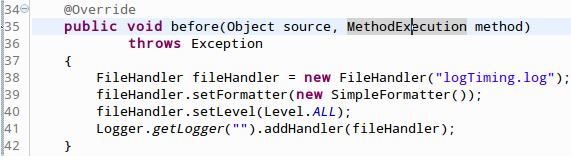
\includegraphics[scale=0.6]{figuras/estudo/loggertimingbefore.png}
	\caption{Implementação do \textit{advice} \texttt{before} do aspecto \texttt{LoggerTiming}.}
	\label{fig:loggeraspectbefore}
\end{figure}

Já o \textit{advice} \texttt{before} possui a função de ativar o armazenamento das informações de \textit{log} em um arquivo, para realização de futuras análises. O arquivo de \textit{log} será criado na pasta raiz do projeto com o nome de \texttt{logTiming.log}.

\subsection{Criação das anotações de extensão}

Para realizar a comunicação entre o aspecto e as classes é necessário utilizar as anotações nativas, ou criar anotações de extensão. Neste estudo de caso optou-se por criar anotações de extensão por ser uma forma mais descritiva e de melhor entendimento, que facilita a leitura do código fonte.

Na figura \ref{fig:extensionenablelog} e \ref{fig:extensionlogtiming} é demonstrada a criação das anotações \texttt{EnableLogInFile} e \texttt{LogTiming}, respectivamente.

\begin{figure}[ht]
	\centering
	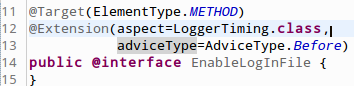
\includegraphics[scale=0.6]{figuras/estudo/extensionenablelog.png}
	\caption{Criação da anotação de extensão \texttt{EnableLogInFile}.}
	\label{fig:extensionenablelog}
\end{figure}

A anotação de extensão \texttt{EnableLogInFile} será utilizada para realizar a comunicação entre o \textit{advice} \texttt{before} do aspecto \texttt{LoggerTiming} e o método \texttt{init} da classe \texttt{Sistema}, com o intuito de ativar o armazenamento das informações de \textit{log} em um arquivo.

\begin{figure}[ht]
	\centering
	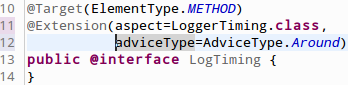
\includegraphics[scale=0.6]{figuras/estudo/extensionlogtiming.png}
	\caption{Criação da anotação de extensão \texttt{LogTiming}.}
	\label{fig:extensionlogtiming}
\end{figure}

Por outro lado a anotação de extensão \texttt{LogTiming} irá ser utilizada nos métodos que terão o tempo calculado, ou seja, os métodos responsáveis pelo carregamento dos módulos.

\subsection{Utilizando anotações de extensão}

As anotações de extensão serão utilizadas para realizar a comunicação do aspecto com o método interceptado. Na figura \ref{fig:usingenablelog} é mostrado a utilização da anotação \texttt{EnableLogInFile}.

\begin{figure}[ht]
	\centering
	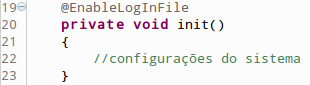
\includegraphics[scale=0.7]{figuras/estudo/initSistema.png}
	\caption{Utilizando a anotação de extensão \texttt{EnableLogInFile}.}
	\label{fig:usingenablelog}
\end{figure}

Neste estudo de caso foi utilizado a anotação \texttt{EnableLogInFile} no método \texttt{init} da classe \texttt{Sistema}, para indicar que antes da inicialização do sistema deve-se ativar o armazenamento em arquivo de \textit{log}.

\begin{figure}[ht]
	\centering
	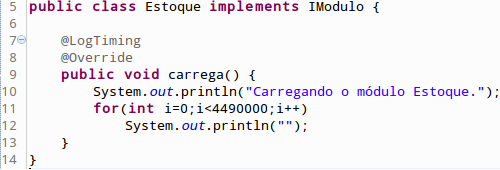
\includegraphics[scale=0.7]{figuras/estudo/modulo.png}
	\caption{Utilização da anotação \texttt{LogTiming} no método \texttt{carrega}.}
	\label{fig:usinglogtiming}
\end{figure}

Foi utilizada a anotação \texttt{LogTiming} no método \texttt{carrega} de todos os módulos (\texttt{Estoque, Caixa e Financeiro}) do sistema. O método \texttt{carrega} foi implementado de forma hipotética em todos os módulos, para isso utilizou-se um \textit{loop} para simular o tempo em que o método ficar executando.

\section{Execução do sistema}

Após realizar a comunicação entre o(s) aspecto(s) e as classes, já é possível executar o sistema. Para isso deve-se compilar o projeto, acessar a pasta \texttt{bin} e executar o seguinte comando para iniciar o sistema utilizando o \textit{framework} para realização da combinação:

\begin{center}
\texttt{java -javaagent:../dist/agent.jar System.Main -classpath ../lib/javassist.jar}
\end{center}

O arquivo \textit{.jar} que representa o \textit{framework} deve estar localizado na pasta \texttt{dist} e a biblioteca Javassist utilizada pelo \textit{framework} deve estar na pasta \texttt{lib}, ambas dentro do projeto, pois são dependências necessárias para a realização da combinação durante o carregamento das classes.

Após a execução do estudo de caso é criado o arquivo de \textit{log} dentro da pasta do projeto, caso ele ainda não exista. A figura \ref{fig:saidaarquivolog} mostra uma das saídas do arquivo de \textit{log} obtidas durante o carregamento dos módulos do sistema.

\begin{figure}[ht]
	\centering
	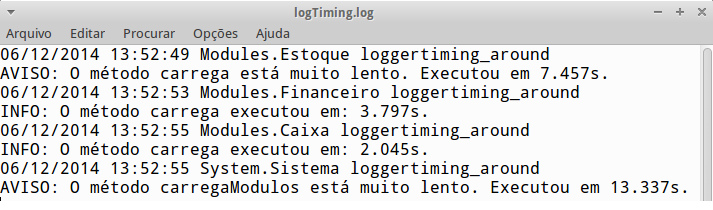
\includegraphics[scale=0.5]{figuras/estudo/saidaarquivolog.png}
	\caption{Saída do arquivo de \textit{log} após o carregamento dos módulos.}
	\label{fig:saidaarquivolog}
\end{figure}

Pode-se perceber que o módulo que demorou mais a carregar foi módulo de \texttt{Estoque} que levou 7.457 segundos em seu carregamento, sendo que o tempo total de carregamento dos módulos do sistema foi de 13.337 segundos.

\section{Considerações finais}

Este capítulo focou no projeto e implementação de um estudo de caso, que utilizou um sistema hipotético para demonstrar a criação e utilização de aspectos no encapsulamento de interesses transversais de um sistema, visando comprovar a eficiência do \textit{framework} desenvolvido na resolução deste problema. Também foi abordado neste capítulo a forma como é feita a comunicação entre aspectos e classes de forma simples com a utilização do \textit{framework}.

\chapter{Conclusão}

\section{Trabalhos futuros}


\singlespacing

\bibliography{bibliografia}

\chapter*{Glossário}

\begin{description}
	\item[SoC] é um princípio de projeto, criado com a finalidade de subdividir o problema em conjuntos de interesses tornando a resolução do problema mais fácil.Cada interesse fornece uma funcionalidade distinta, podendo ser validado independentemente das regras negócio \cite{pressman2010engineering}.
	\item [YAGNI] é um princípio de projeto, bastante usado em equipes XP , cuja principal finalidade é implementar apenas o necessário.
	\item[Extreme Programming] XP é um estilo de desenvolvimento de software com foco em excelentes técnicas de programação, comunicação clara e trabalho em equipe, que permite grande produtividade no desenvolvimento \cite{beck2004extreme}.
\item [Decorator] é um padrão de projeto estrutural, cujo principal objetivo é adicionar funcionalidades a um objeto dinamicamente.
\item [Proxy] é um padrão de projeto estrutural, cujo principal objetivo é controlar as chamadas a um objeto através de outro objeto de mesma interface.
\item [Log] é o arquivo onde é registrado informações relevantes sobre o comportamento do sistema \cite{log}.
\end{description}

\appendix

\chapter{Versão completa dos diagramas}
\label{apend:A}

\end{document}

